\section{Določevanje frekvenčnega spektra}

Frekvenčni spekter lahko določimo na različne načine. V tem poročilu se osredotočamo na Metodo maksimalne entropije (MME), za primerjavo pa podajam tudi rezultate bolj uveljavljene hitre Fourirove transformacije (FFT). Zavoljo preglednosti so prikazane le pozitivne frekvence. Spekteralno gostoto moči (PSD) se po MME določi
\begin{equation}
    PSD(\omega) = |H(e^{i\,\omega})|^2 = \frac{G^2}{|a + \sum_{k=1}^{p} a_k\, e^{-i\,\omega}|^2},
\end{equation}
kjer je $p$ red filtra, $H(z) = S(z)/U(z)$ kompleksna prenosna funkcija in $G$ ter $a_k$ parameteri, ki se določijo iz podatkov. Ker uporabljamo avtoregresijski model, imamo v števcu prenosne funkcije same ničle, parametre filtra lahko določimo iz reševanja Yule-Walkerjevega sistema enačb ob avtokorelaciji signala $R(i)$, kjer predpostavimo stacionaren proces:
\begin{equation}
    \sum_{k=1}^{p} a_k\, R(|i-k|) = -R(i), \quad 1 \leq i \leq \infty.
\end{equation}
Parameter $G$ se izračuna po enačbi
\begin{equation}
    G^2 = R(0) + \sum_{k=1}^{p} a_k\, R(k)
\end{equation}
in predsatvalja oceno šuma v meritvah.

Za izračun PSD spektra sem uporabljal funkcijo \texttt{pyule} iz Python modula \texttt{spectrum}, ki je sorodna funkciji \texttt{aryule}.

\subsection{Testni signali}

Kot prvo preverim delovanje na testenem sinusu. MME zazana frekvenco, tako kot FFT, vendar je vrednost PSD manjša od FFT. Prav tako se niža z večanjem števila polov.

\begin{figure}[ht]
    \centering
    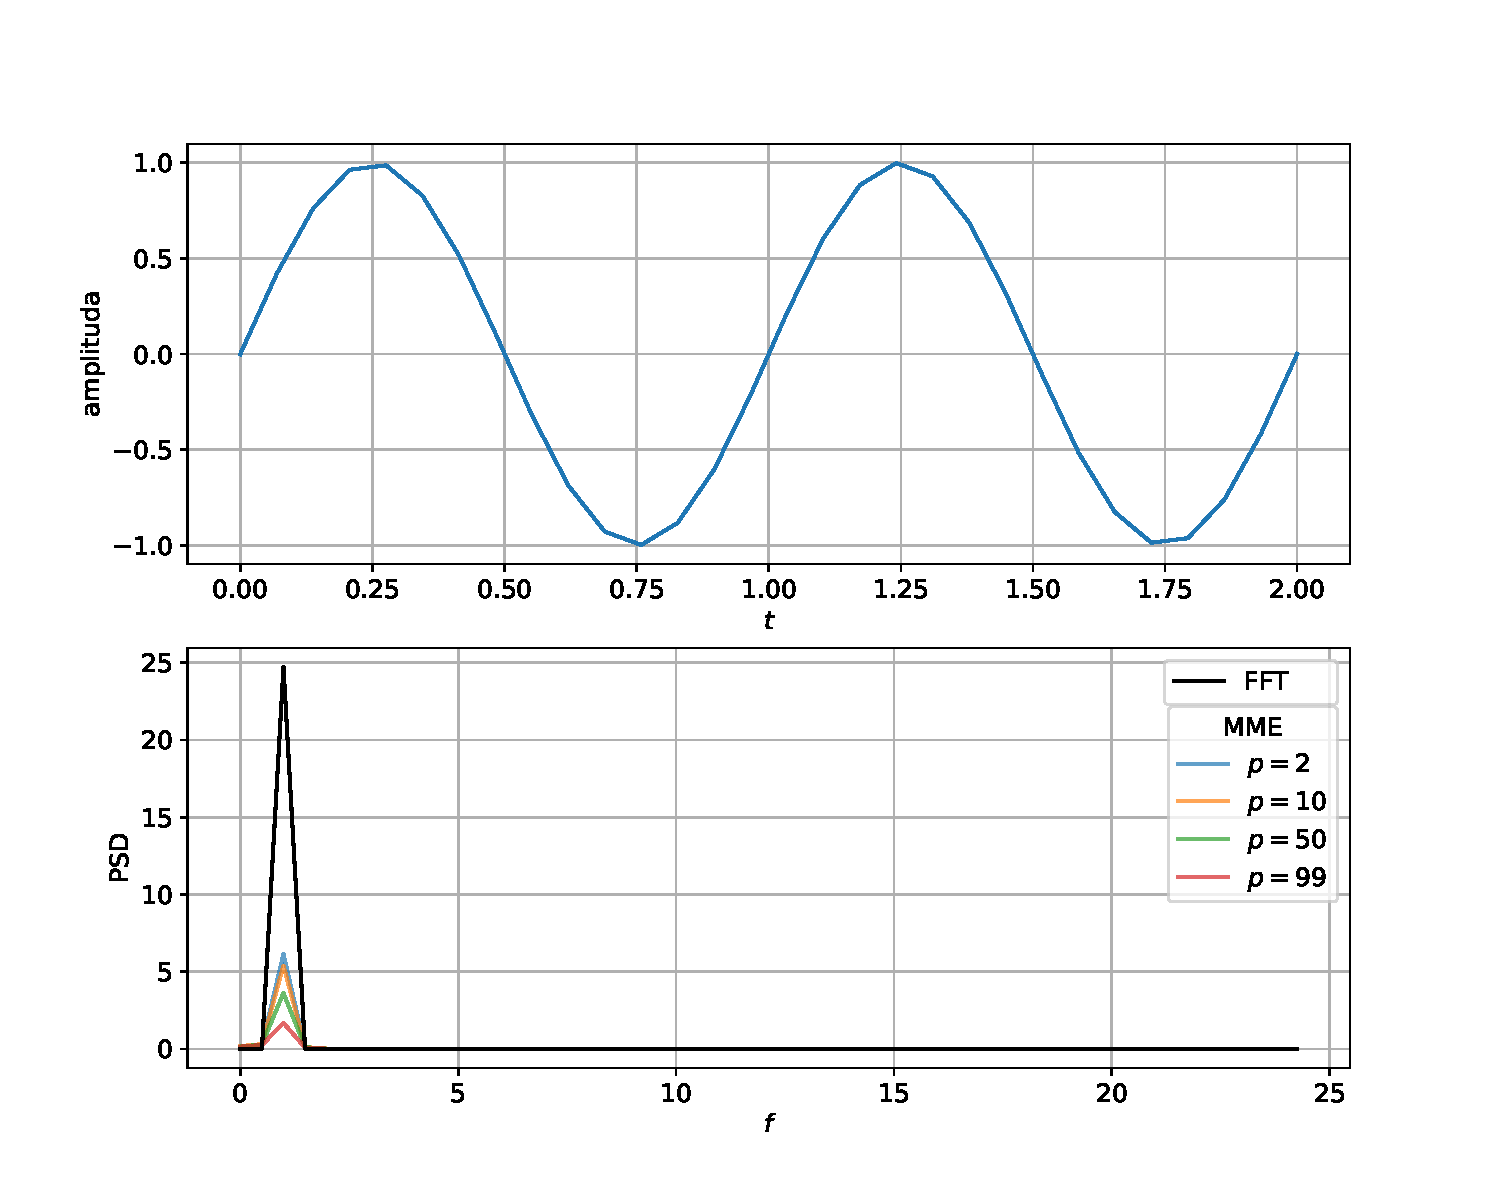
\includegraphics[width=0.5\textwidth]{12.nal_slike/12.1/test_sin.pdf}
    \caption[short]{Testni sinusni signal s frekvenco 1 Hz}
\end{figure}

Poizkusimo analizirati tudi vsoto dveh sinusov bližnjih frekvenc. Dobimo signal, ki ustreza amplitudni modulaciji (AM) sinusnega signala z modulacijsko frekvenco $f_{mod}$ in simusnega nosilnega (carrier) signala s frekvenco $f_c$. Ti dve frekvenci lahko preprosto izračunamo iz obeh sestavnih frekvenc signala $f_1$ in $f_2$:
\begin{equation}
    f_{mod} = \frac{|f_1-f_2|}{2}, \quad f_c = \frac{f_1+f_2}{2}.
\end{equation}
Opazimo, da FFT in MME ne zaznata niti modulacijske, niti nosilne, ampak obe sestavni frekvenci signala. Čudno je le to, da sta jakosti frekvenc različni. Če pa še bolj približamo sestavni frekveci signala, pa ju metodi zaradi premajahne frekvečne ločljivosti ne loči.

\begin{figure}[ht]
    \centering
    \begin{subfigure}{0.49\textwidth}
        \centering
        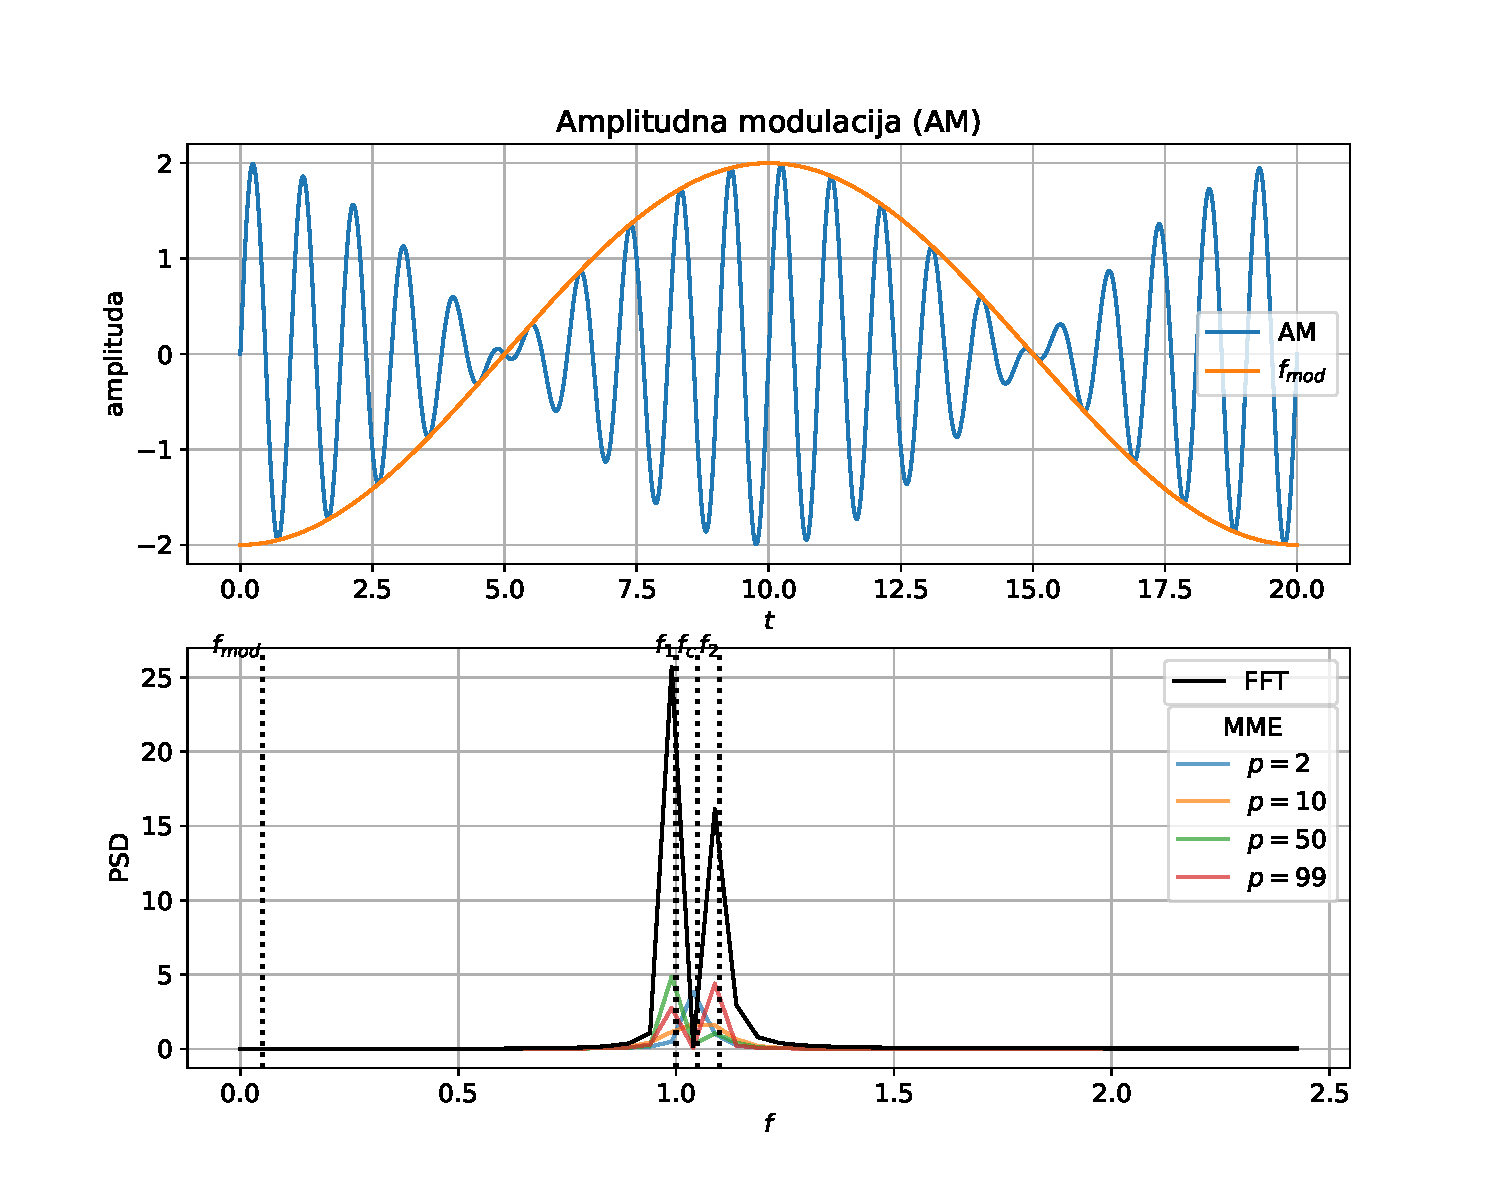
\includegraphics[width=\textwidth]{12.nal_slike/12.1/AM.pdf}
        \caption[short]{}
    \end{subfigure}
    \begin{subfigure}{0.49\textwidth}
        \centering
        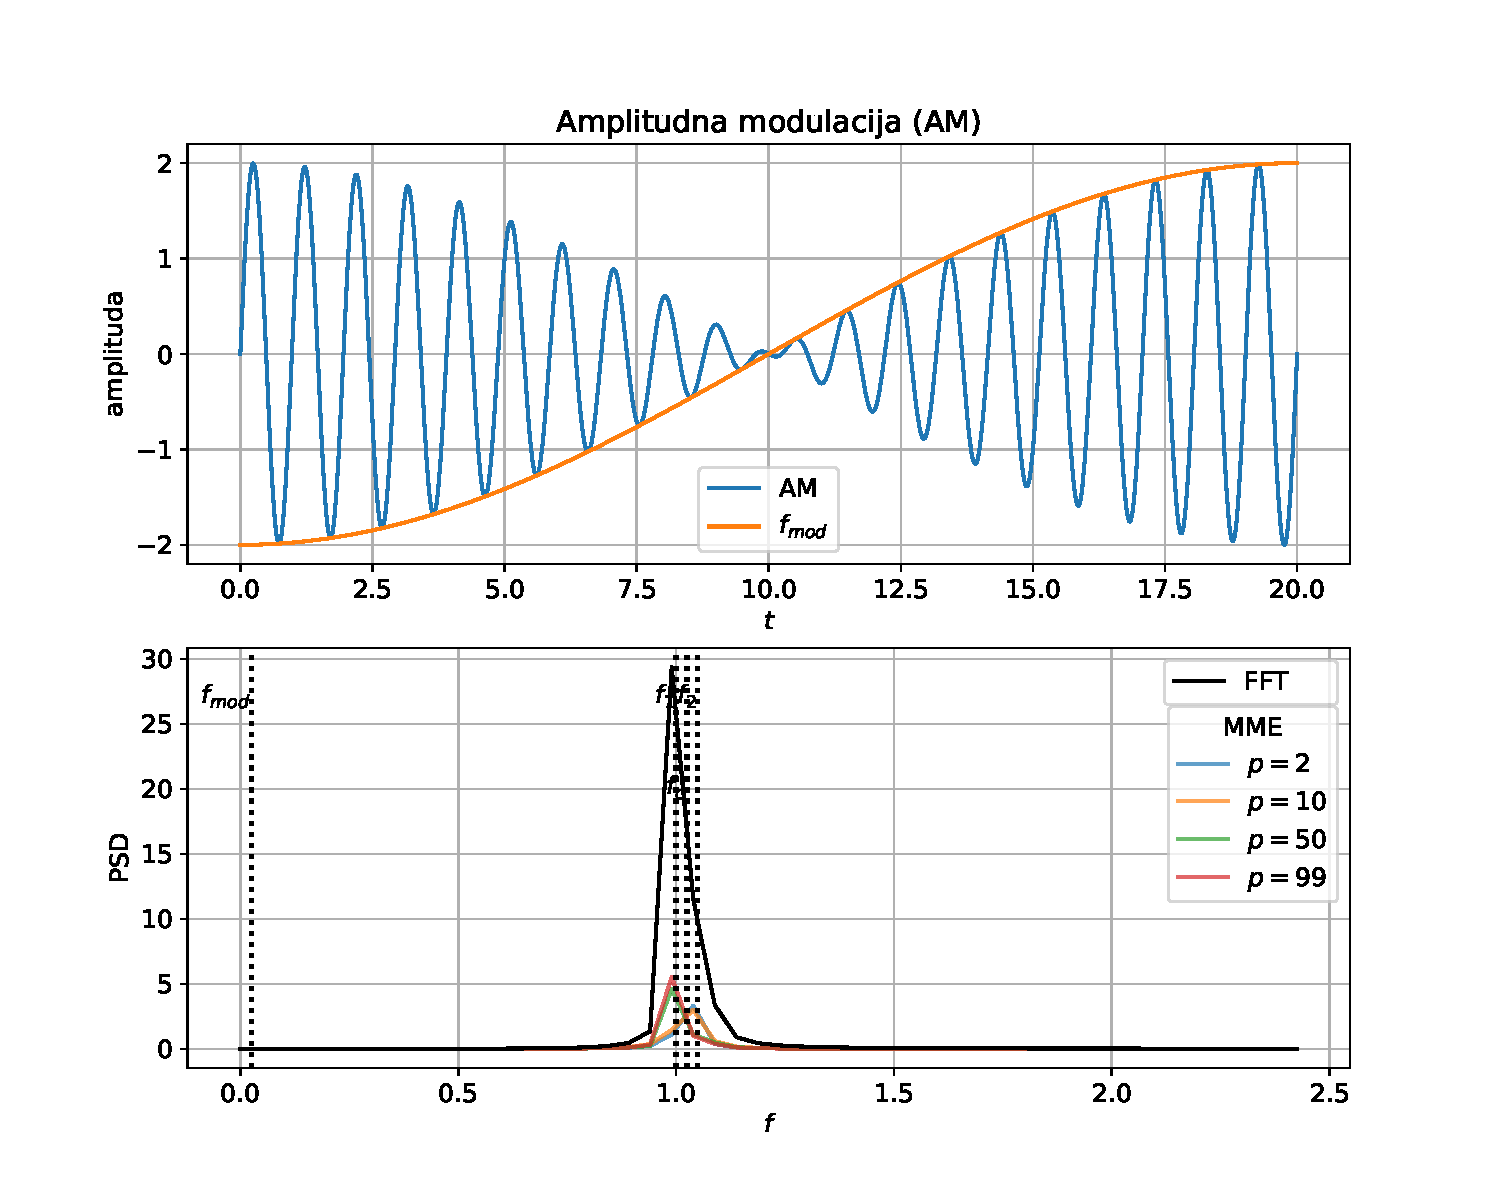
\includegraphics[width=\textwidth]{12.nal_slike/12.1/AM_še_bližnji_freq.pdf}
        \caption[short]{}
    \end{subfigure}
    \caption[short]{Testni signal dveh sinusov bližnjih frekvenc (a)(1 in 1,1) in (b)(1 in 1,05)}
\end{figure}

\newpage
Preizkusil sem tudi preostali dve modulaciji signala, kjer spektralne metode odpovejo pri iskanju modulacijske/nosilne frekvence. Le pri FM se izkaže, da je spekter simetričen glede na $f_c$, kar je verjetno odraz nihanja frekvence signala. Pri frekvečni modulaciji je nosilna frekvenca $f_c=10$ in modulacijski indeks $k_f=2$, pri fazni pa $f_c=1$.

\begin{figure}[H]
    \centering
    \begin{subfigure}{0.49\textwidth}
        \centering
        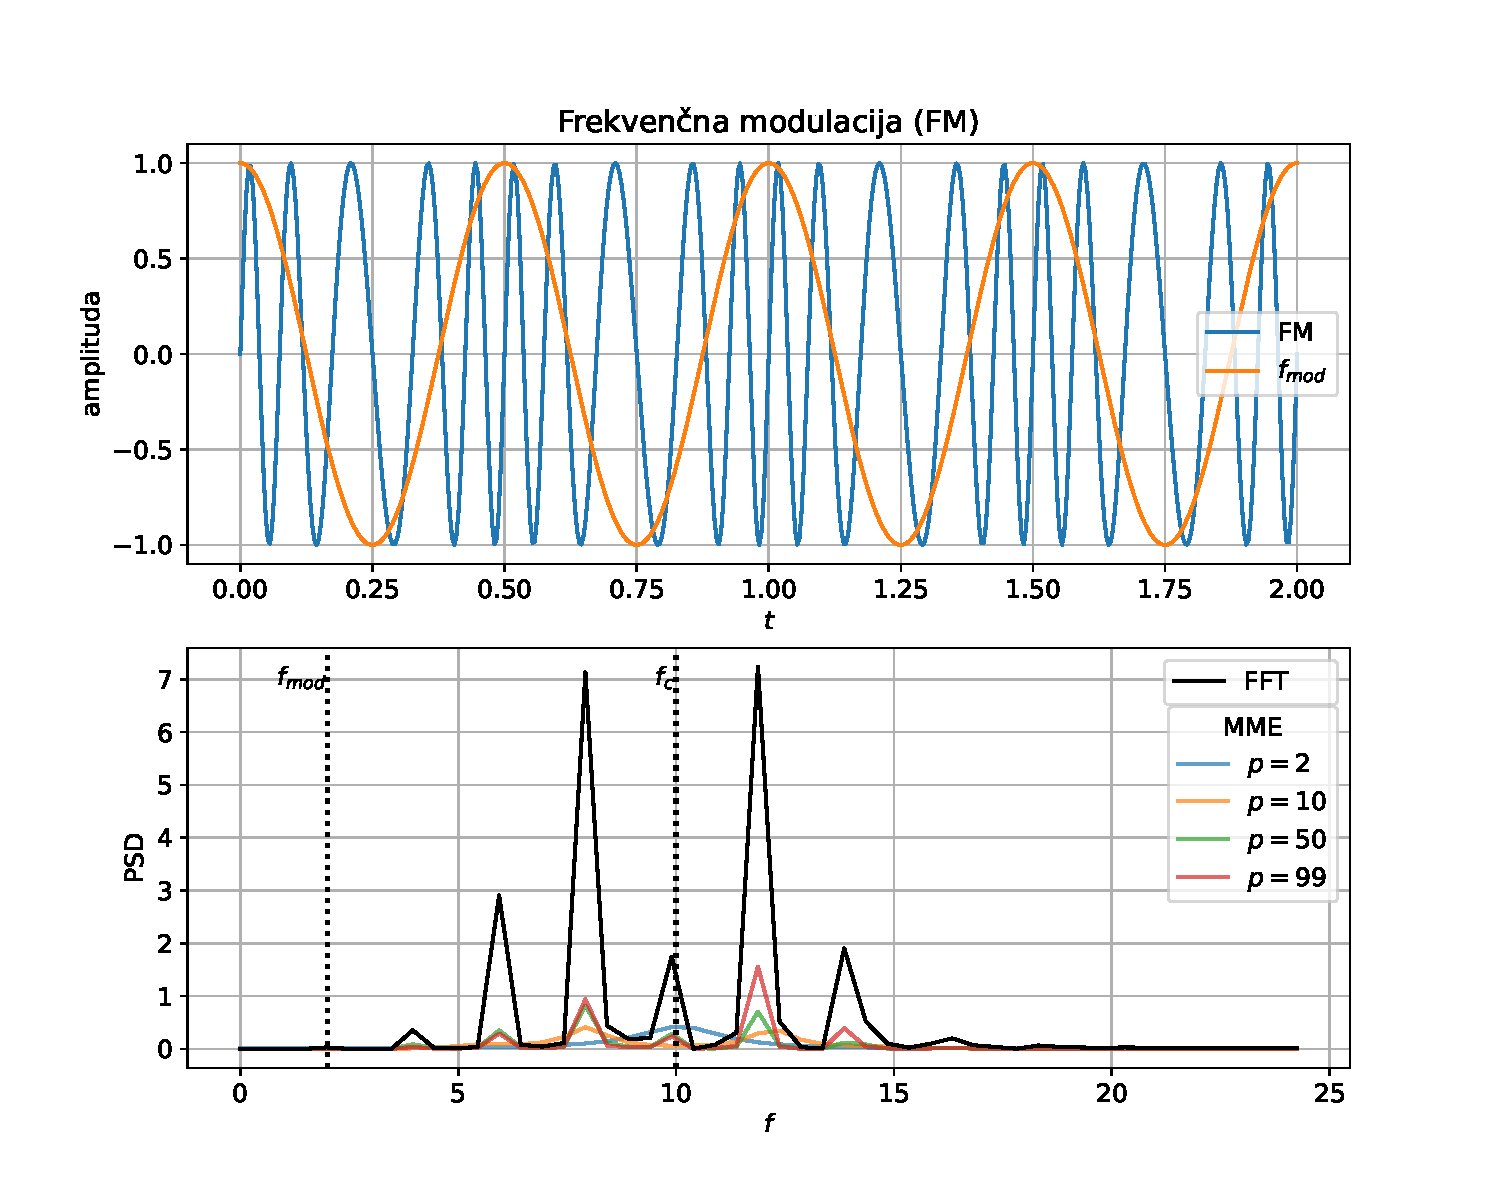
\includegraphics[width=0.75\textwidth]{12.nal_slike/12.1/FM.pdf}
        \caption[short]{}
    \end{subfigure}
    \begin{subfigure}{0.49\textwidth}
        \centering
        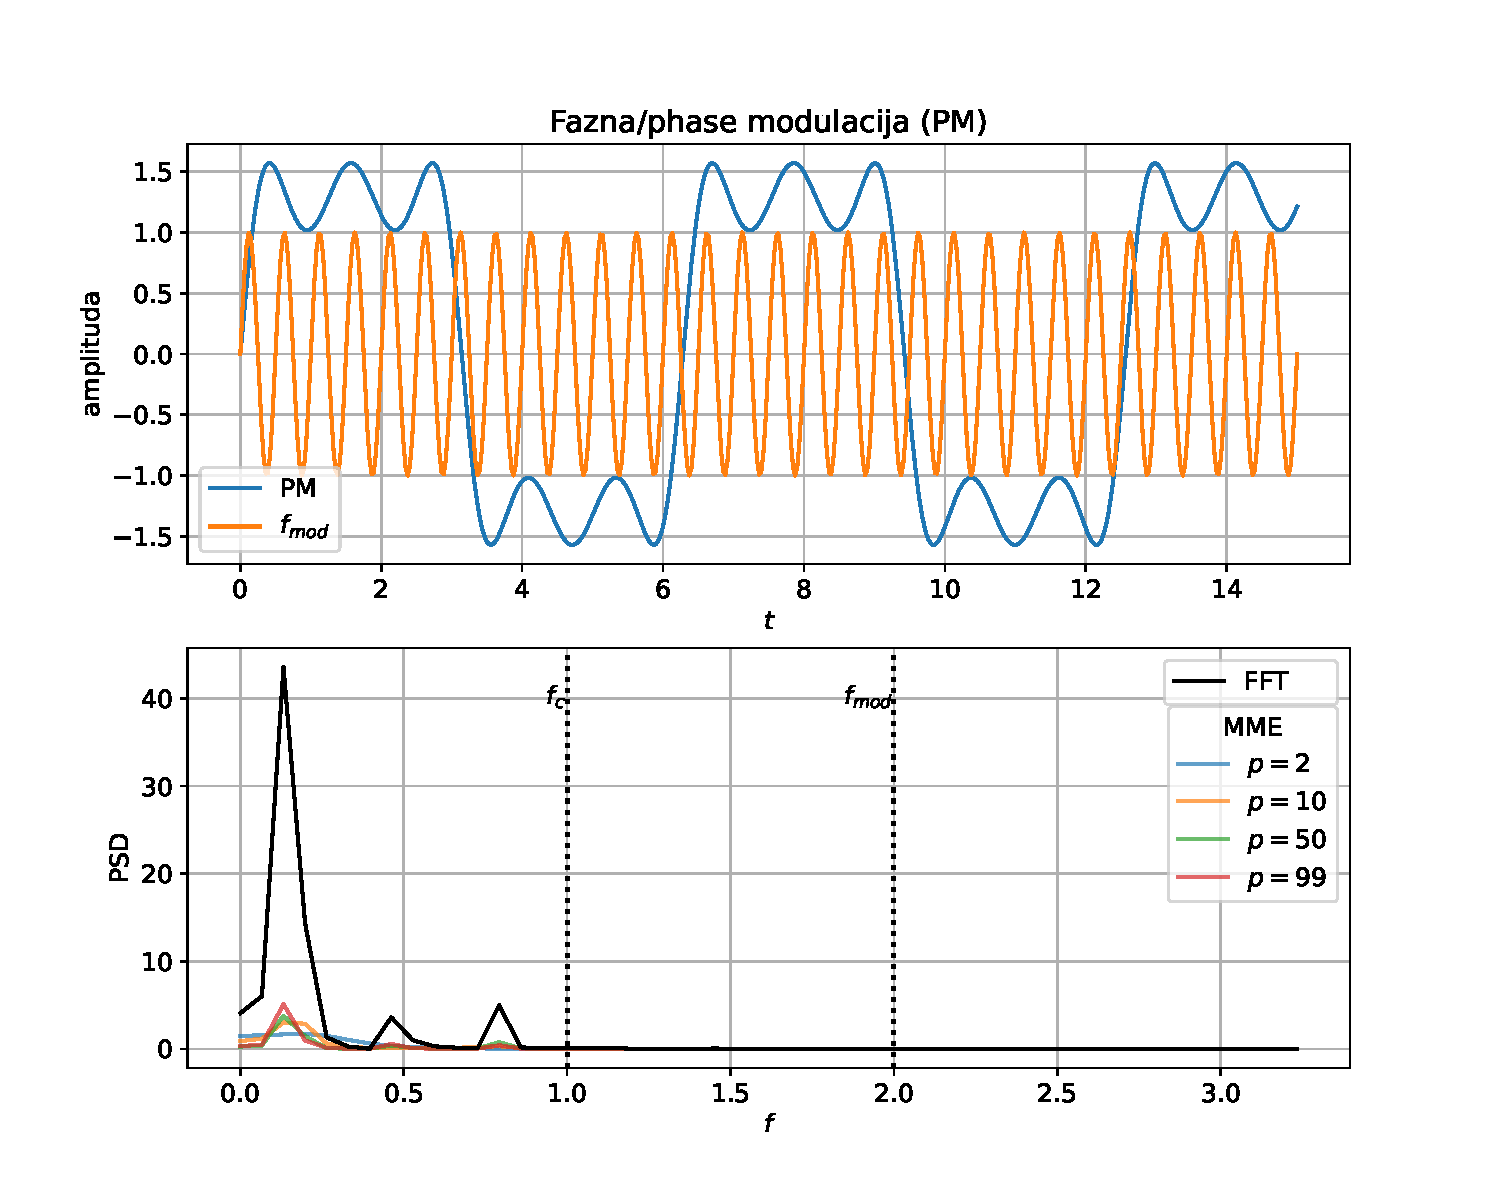
\includegraphics[width=0.75\textwidth]{12.nal_slike/12.1/PM.pdf}
        \caption[short]{}
    \end{subfigure}
    \caption[short]{Testni signal (a) frekvenčne in (b) fazne modulacije $f_{mod}=2$}
\end{figure}

\newpage
\subsection{Podatki iz datotek}

Sedaj bomo podrobneje analizirali podatke in pri tem preizkusili tudi večji red filtra  in okenske funkcije. Slednje imajo na MME enak vpliv, kot na FFT, kar je opazno le na signalu val3. Večanje reda privede do večje frekvečne ločljivosti in šele ko je ta dovolj velika, lahko zaznamo vrh pri vsebovani frekvenci. Največji možen red je enak dimenziji signala, v takem primeru je spekter zelo podoben FFT, če odmislimo drugačne amplitude. Na sliki je sicer prikazano le do reda 14, s katerim pa lahko že dovolj dobro analiziramo signale. Velja poudariti, da večanje reda ob hkratni uporabi okenske funkcije izničuje učinke puščanja, medtem ko to brez okna ni tako izrazito za višje rede.

\begin{figure}[ht]
    \centering
    \begin{minipage}{0.49\textwidth}
        \centering
        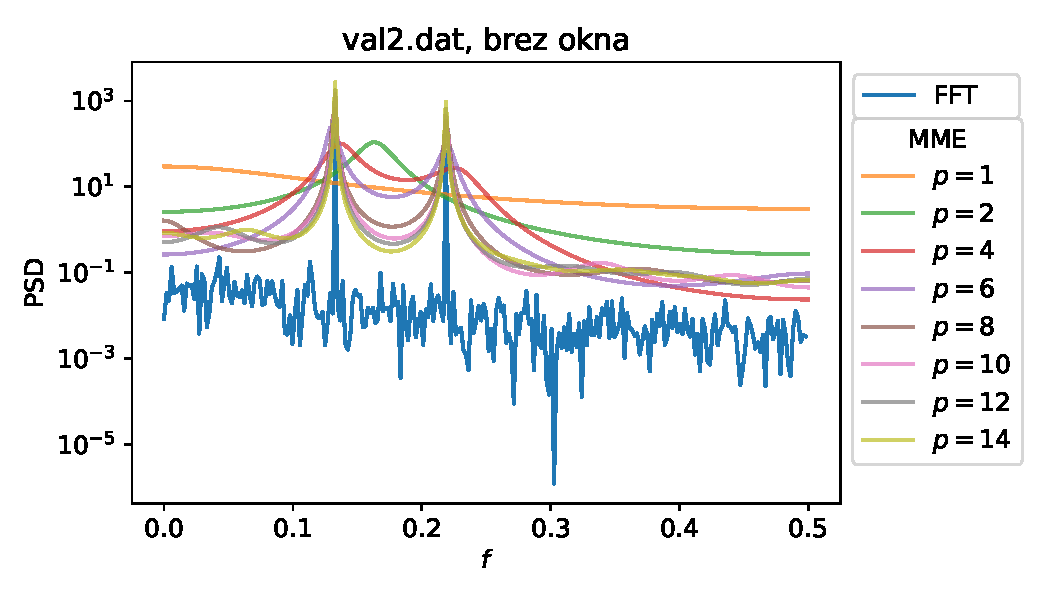
\includegraphics[width=\linewidth]{12.nal_slike/12.1/PSD_val2.pdf}
    \end{minipage}
    \begin{minipage}{0.49\textwidth}
        \centering
        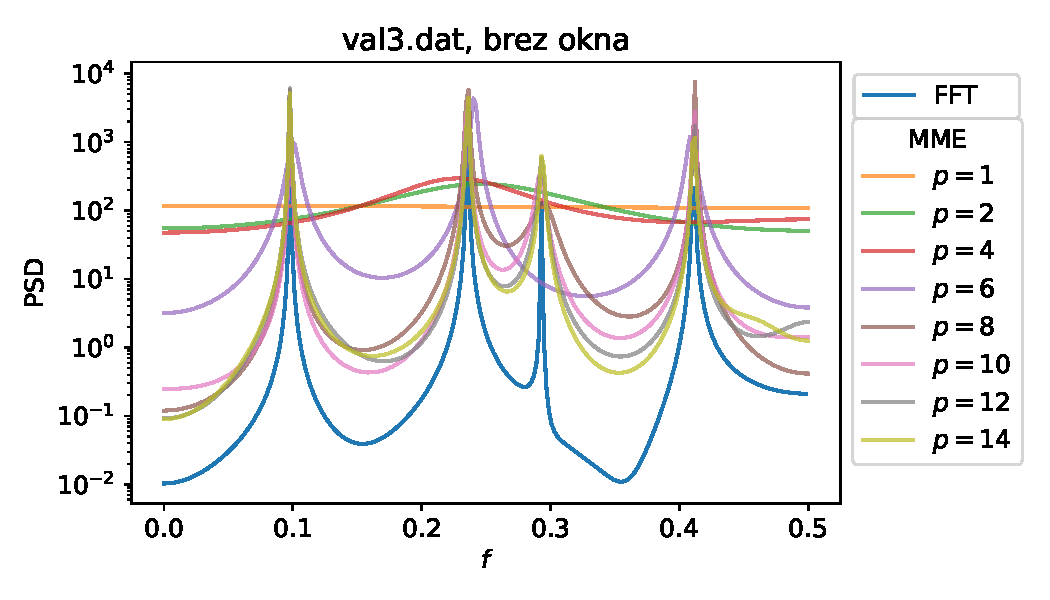
\includegraphics[width=\linewidth]{12.nal_slike/12.1/PSD_val3.pdf}
    \end{minipage}
    \caption[short]{PSD datotek brez okna}
\end{figure}

\begin{figure}[ht]
    \centering
    \begin{minipage}{0.49\textwidth}
        \centering
        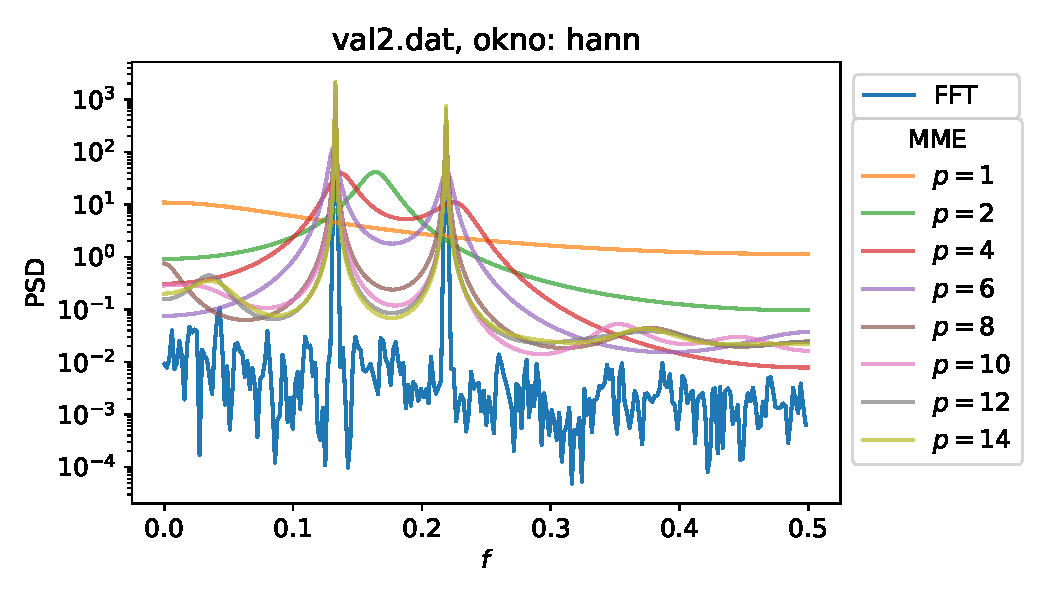
\includegraphics[width=\linewidth]{12.nal_slike/12.1/PSD_val2_hann.pdf}
    \end{minipage}
    \begin{minipage}{0.49\textwidth}
        \centering
        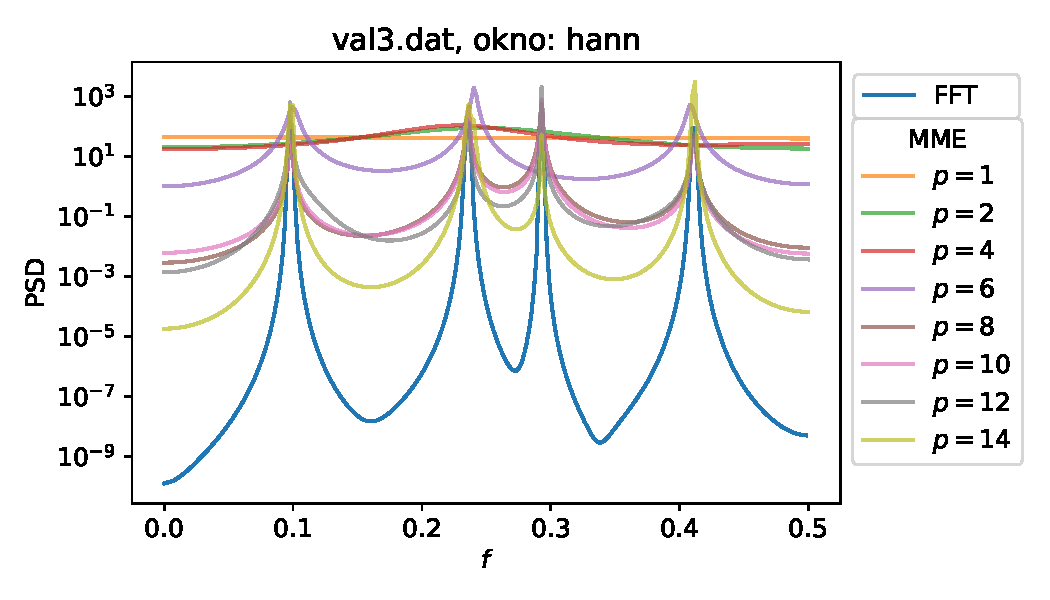
\includegraphics[width=\linewidth]{12.nal_slike/12.1/PSD_val3_hann.pdf}
    \end{minipage}
    \caption[short]{PSD datotek z oknom Hann}
\end{figure}

Za analizo podatkov iz datoteke co2.dat, je potrebno najprej popraviti podatke. Vrednosti, ki predstavljajo odsotnost meritev, sem preprosto odstranil iz signala. Ker je manjkajočih podatkov tako malo, to ne vpliva bistveno na anlizo. Prav tako sem izračunal linearni letni trend koncentracij in ga odštel od signala, kar je vidno na spodnji sliki.

\begin{figure}[ht]
    \centering
    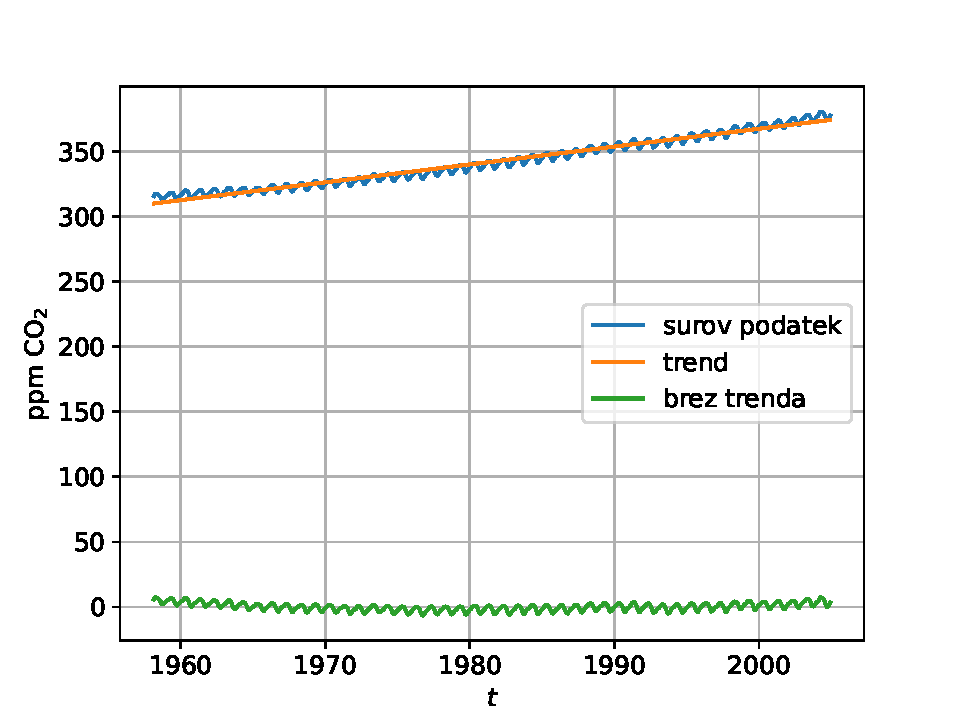
\includegraphics[width=0.4\textwidth]{12.nal_slike/12.1/co2_potek_trend.pdf}
    \caption[short]{Podatki iz datoteke \texttt{co2.dat} upoštevajoč linearen trend}
\end{figure}

Opazim, da okno očitno pripomore k izboljšanju spektra, saj se odpravi oscilacije in tako omogoči, da zaznamo (sicer majhne) vrhove frekvenc pri 1 in 2 na leto. Ko odštejemo linearen trend so te letne oscilacije bolj izrazite, pri MME je za to potreben red, večji od 10. Zanimivo je, da tukaj ni več opazne ``doline'' okoli frekvence 4, kar si ne znam pojasniti iz podatkov.

\begin{figure}[ht]
    \centering
    \begin{minipage}{0.49\textwidth}
        \centering
        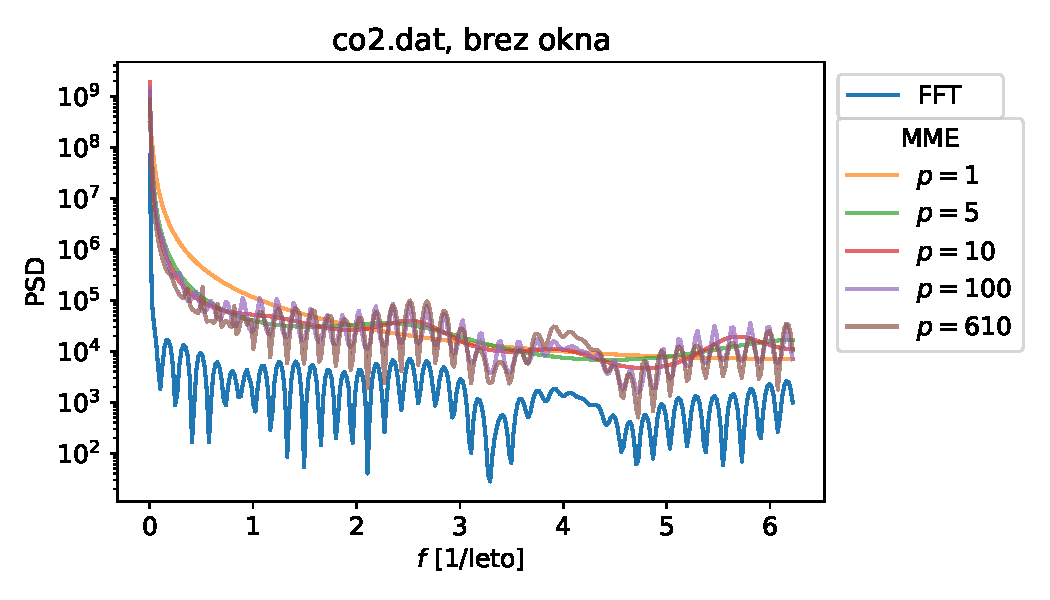
\includegraphics[width=\linewidth]{12.nal_slike/12.1/PSD_co2_.pdf}
    \end{minipage}
    \begin{minipage}{0.49\textwidth}
        \centering
        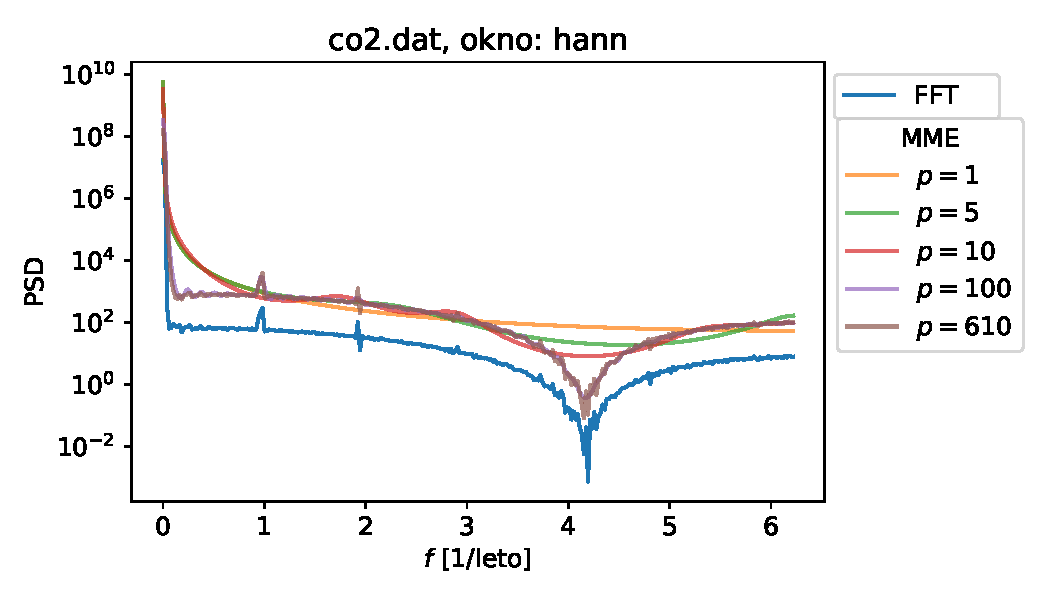
\includegraphics[width=\linewidth]{12.nal_slike/12.1/PSD_co2_hann.pdf}
    \end{minipage}
    \caption[short]{PSD datoteke \texttt{co2.dat}}
\end{figure}

\begin{figure}[ht]
    \centering
    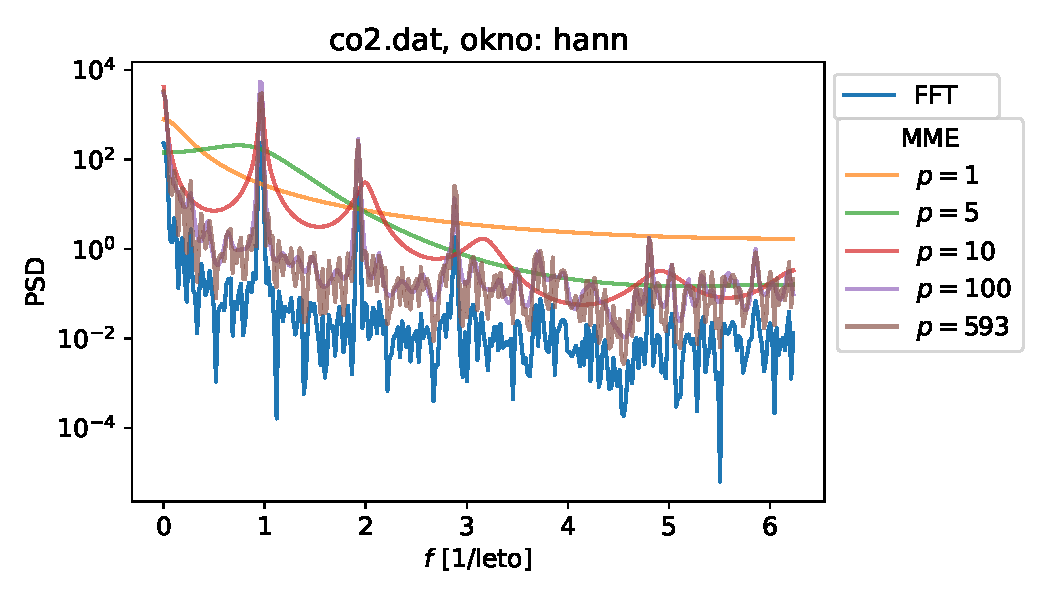
\includegraphics[width=0.5\linewidth]{12.nal_slike/12.1/PSD_co2_trend_hann.pdf}
    \caption[short]{PSD datoteke \texttt{co2.dat} upoštevajoč linearen trend}
\end{figure}

Sedaj si lahko pogledamo tudi tako zvano napako metode MME, glede na FFT. Na spodnjih treh slikah je prikazana relativna napaka, kjer je absolutna vrednost pogreška med metodama deljena z vrednostjo FFT pri različnem redu filtra. Opazimo lahko podobne zaključke kot iz zgornjih grafov: v splošnem večanje reda filtra vodi k manjši napaki, vendar z iskanjem minimuma ugotovimo, da temu ni vedno tako. Obstajajo tudi lokalni minimumi, ki so hkrati tudi globalni! V takem primeru bi bil to optimalen red. Prikazana logaritmična napaka upošteva log skalo na y-osi.

Opazimo, da smo se pri datoteki val2 z zgornjih grafih zajeli, slabše pa je bilo pri uporabi okenske funkcije, saj nismo uporabili dovolj redov, da bi zmanjšali napako, zato je izgledalo, kot da okenska funkcija nima učinka. Velja pa poudariti, da je njen učinek mnogo večji pri val3 in co2, kjer log napako zmanjšamo celo za (nekaj) redov velikosti, vendar to prinese nihanja pri nižjih redih.

\begin{figure}[ht]
    \centering
    \begin{minipage}{0.49\textwidth}
        \centering
        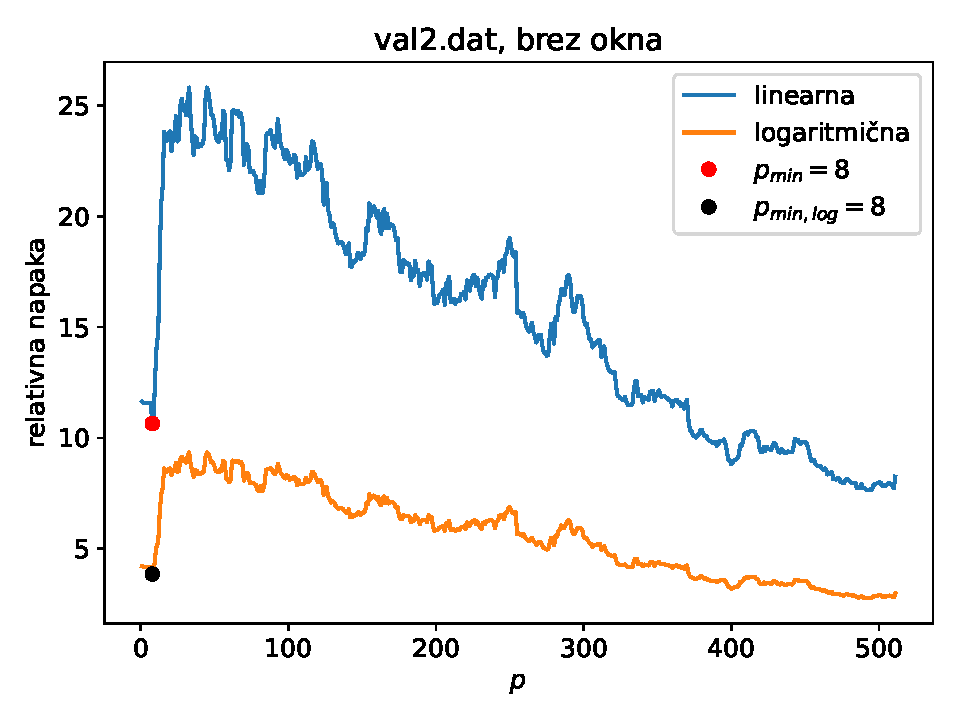
\includegraphics[width=\linewidth]{12.nal_slike/12.1/napaka_val2.pdf}
    \end{minipage}
    \begin{minipage}{0.49\textwidth}
        \centering
        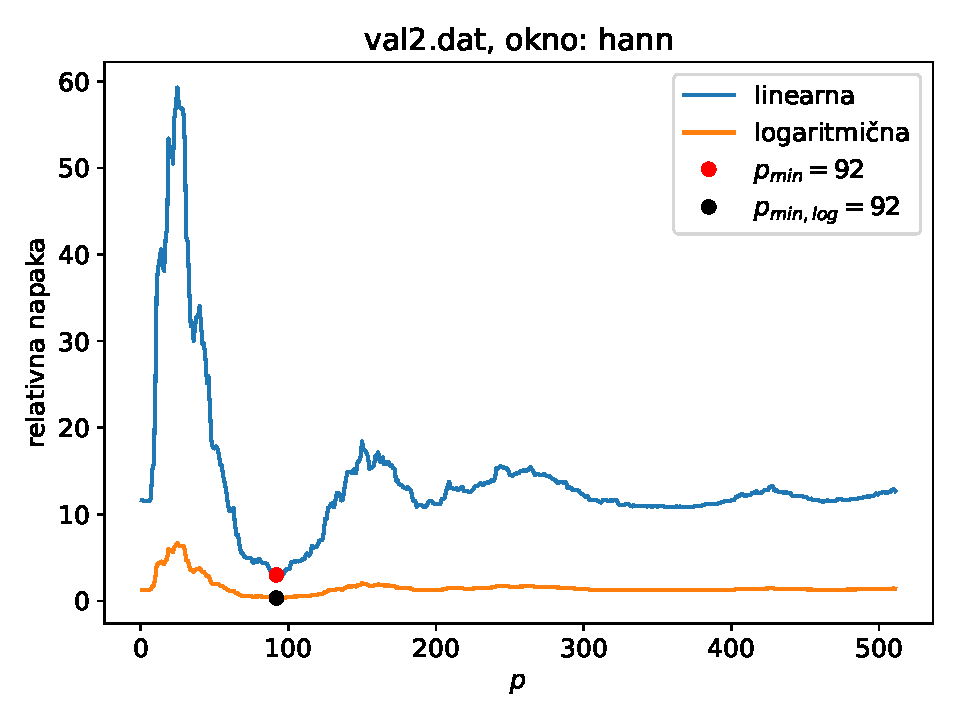
\includegraphics[width=\linewidth]{12.nal_slike/12.1/napaka_val2_hann.pdf}
    \end{minipage}
    \caption[short]{Napaka v odvisnosti od reda filtra $p$ za \texttt{val2}}
\end{figure}

\begin{figure}[ht]
    \centering
    \begin{minipage}{0.49\textwidth}
        \centering
        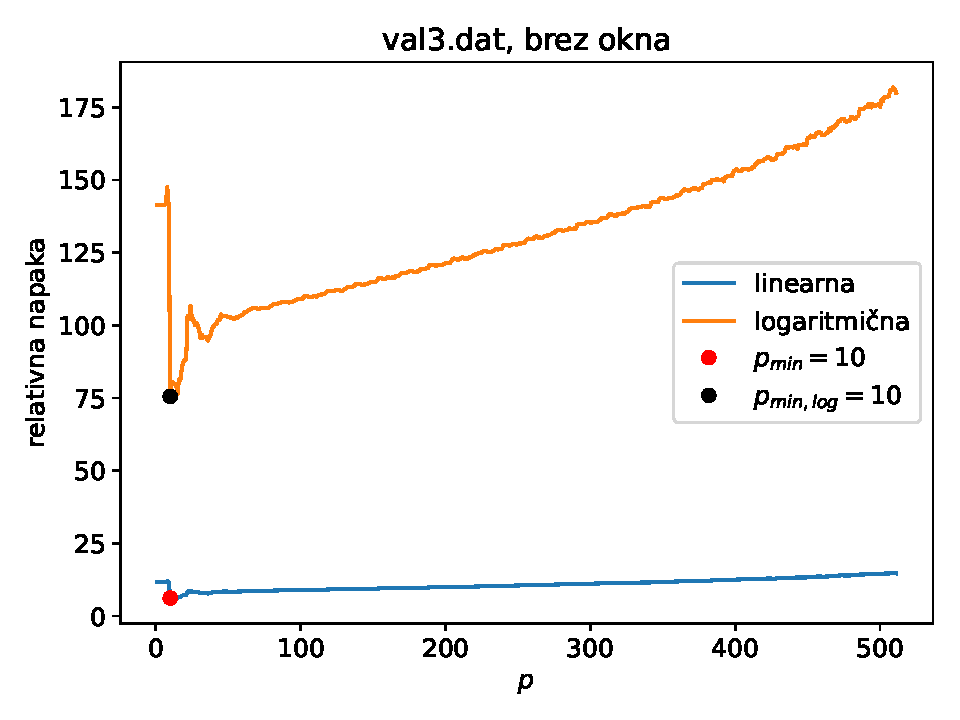
\includegraphics[width=\linewidth]{12.nal_slike/12.1/napaka_val3.pdf}
    \end{minipage}
    \begin{minipage}{0.49\textwidth}
        \centering
        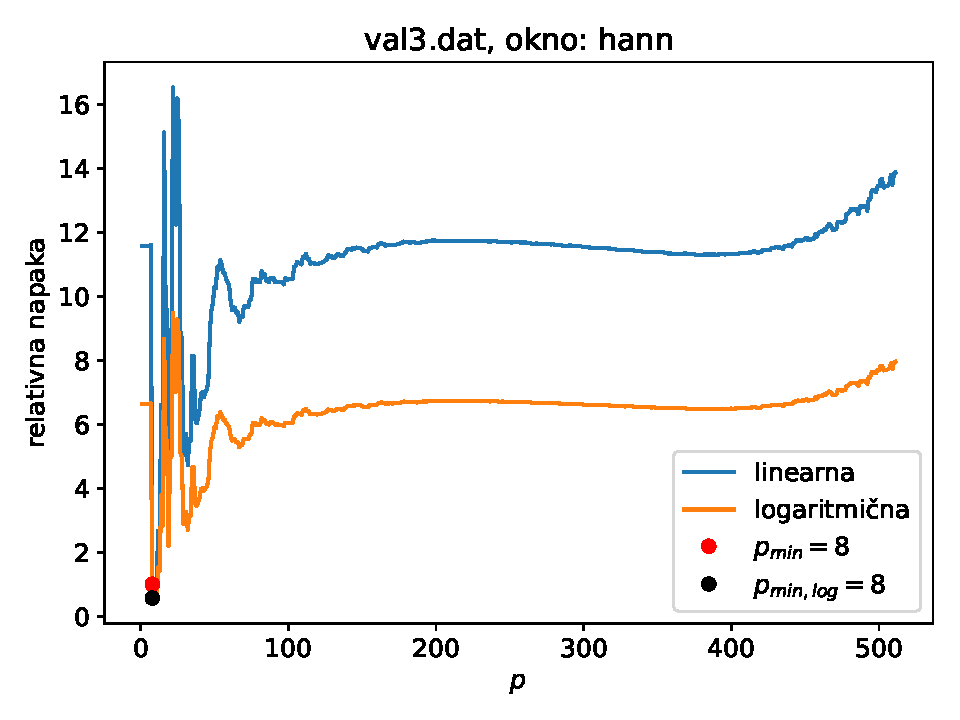
\includegraphics[width=\linewidth]{12.nal_slike/12.1/napaka_val3_hann.pdf}
    \end{minipage}
    \caption[short]{Napaka v odvisnosti od reda filtra $p$ za \texttt{val3}}
\end{figure}

\begin{figure}[ht]
    \centering
    \begin{subfigure}{0.49\textwidth}
        \centering
        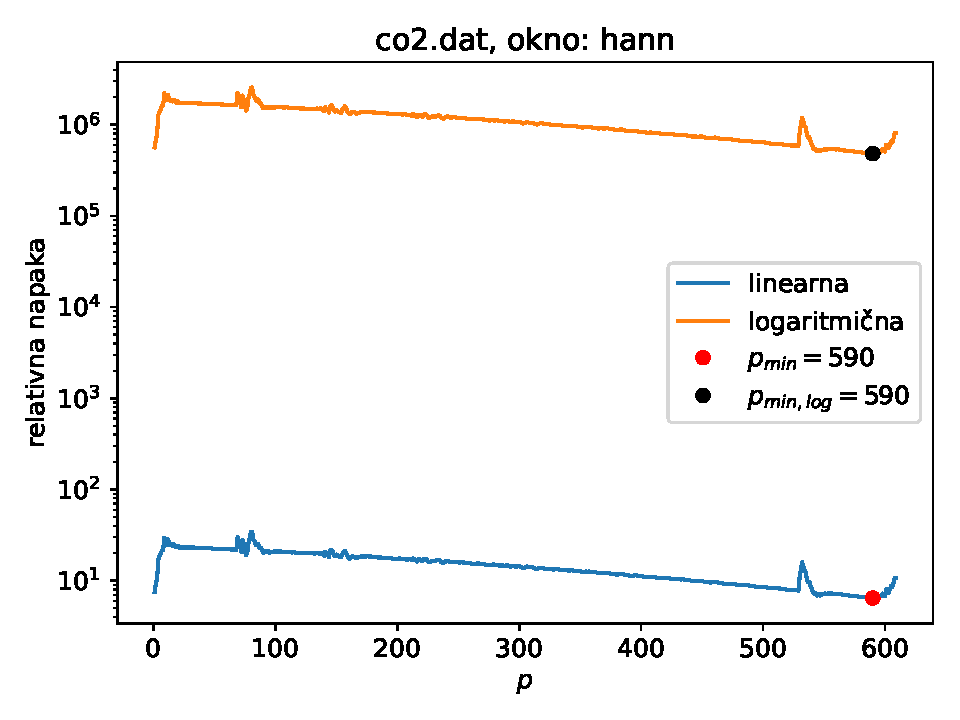
\includegraphics[width=\linewidth]{12.nal_slike/12.1/napaka_co2_hann.pdf}
        \caption[short]{brez trenda}
    \end{subfigure}
    \begin{subfigure}{0.49\textwidth}
        \centering
        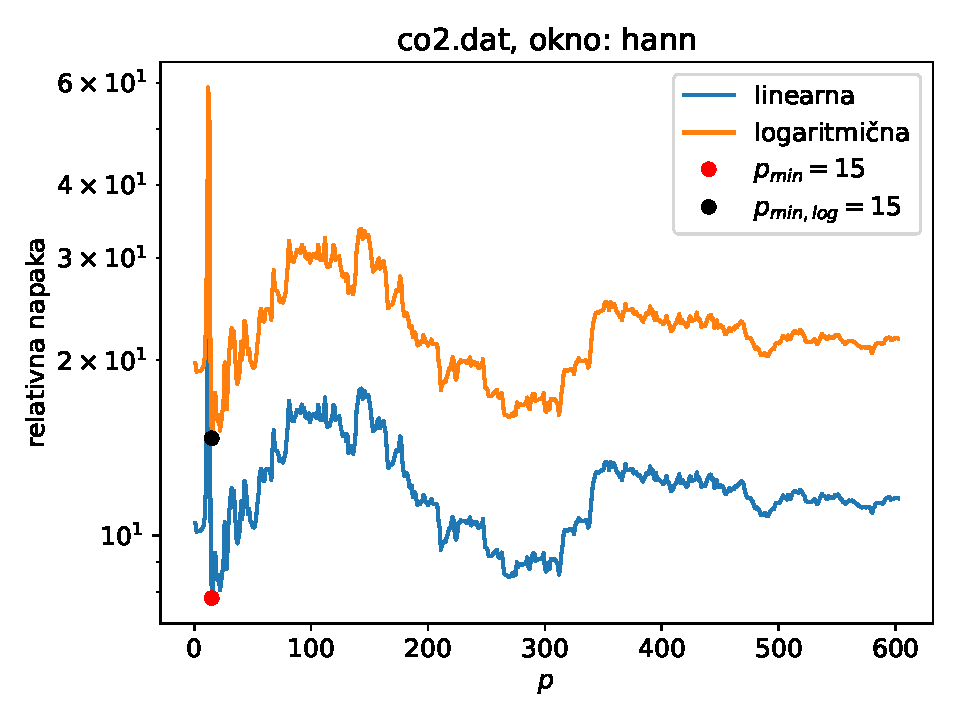
\includegraphics[width=\linewidth]{12.nal_slike/12.1/napaka_co2_trend_hann.pdf}
        \caption[short]{upoštevajoč linearen trend}
    \end{subfigure}
    \caption[short]{Napaka v odvisnosti od reda filtra $p$ za \texttt{co2}}
\end{figure}

\section{Linearna napoved}

Koeficiente $a_k$ iz avtoregresijskega modela lahko uporabimo tudi za linearno napoved. Izračunamo jih iz prve polovice signala, drugo pa uporabimo za referenco. Napovedane vrednosti določamo glede na predhodnje in glede na red filtra $p$ po enačbi:
\begin{equation}
    S_n = -\sum_{k=1}^{p} a_k\, S_{n-k} + G\, u_n,
\end{equation}
kjer so $S_n$ izhodi iz sistema in $u_n$ vhodi.

Tako lahko določimo tudi pole kompleksne preslikave (ničle imenovalca), katerih število je enako redu $p$
\begin{equation}
    1 + \sum_{k=1}^{p} a_k\, z^{-k} = 0.
\end{equation}
Taki poli, ki ležijo izven enotske krožnice na kompleksni ravnini lahko predstavljajo vire nestabilnosti napovedi, zato jih je mogoče preslikati v notranjost ali na krožnico.

Uporabljal sem različne že vgrajene metode v Pythonu kot so \texttt{spectrum.aryule} in \texttt{arburg}, ki namesto Yule-Walkerja uporablja Burg-ov algoritem za oceno parametrov $a_k$, \texttt{statsmodels.regression.linear\_model.yule\_walker}, ki ima dve različni implementaciji ocene avtokorelacijske funkcije (ACF), \textit{adjusted} in \textit{maximum-likehood estimation (MLE)}  ter \texttt{statsmodels.tsa.ar\_model.AutoReg}, ki uporablja \textit{Conditional Maximum Likelihood (OLS)}.

Kot prvo preizkusim delovanje funkcij na testnem sinusnem signalu, kar je prikazno na spodnji sliki. Različne funkcije se obnašajo zalo drugače, vendar jim vsem bolj ali manj uspe izluščiti frekvenco, nekateri pa tudi amplitudo. Opazim, da zrcaljenje polov ne pripomore k bolši rešitvi, temveč celo k slabši, kar mi ni jasno.

\begin{figure}[ht]
    \centering
    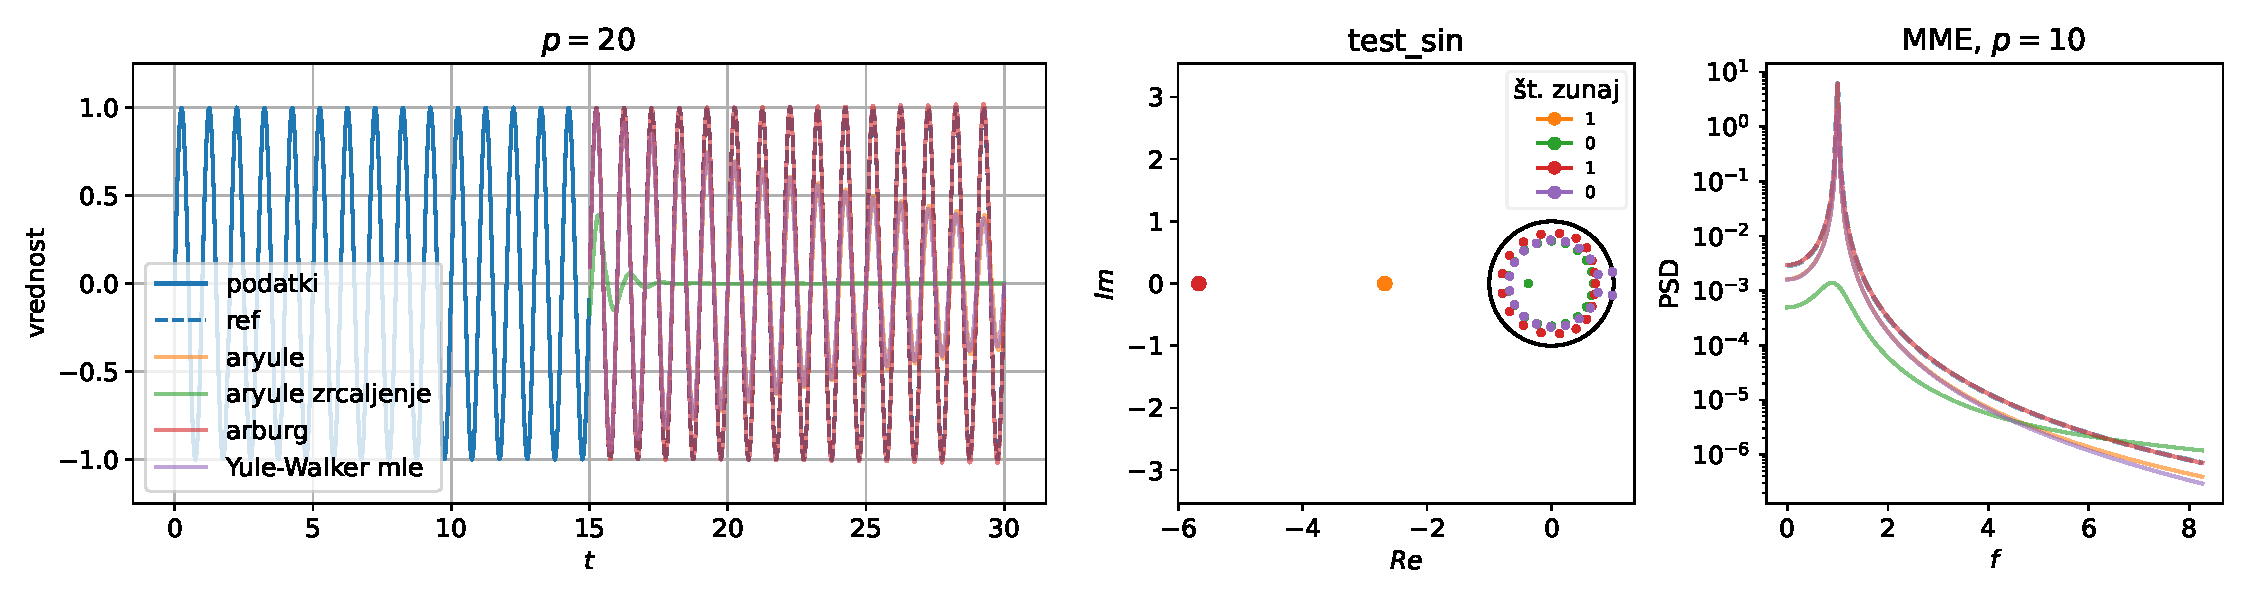
\includegraphics[width=\textwidth]{12.nal_slike/napoved_test_sin.pdf}
    \caption[short]{Testna napoved sinusnega signala}
\end{figure}

\subsection{Signali iz prve naloge}

Na spodnji sliki so prikazane časovna napoved z redom $p=20$, poli in PSD spekter napovedi. Ponovno je opazno, da zrcaljenje ne izboljša rešitve, korelacije med število polov izven enotske krožnice in napako ni moč ugotoviti. Prav tako, sploh pri co2 metode zelo težko ujamejo amplitudo, to še najbolje uspeva funkciji \texttt{yule\_walker}, pri val3 se dobro obnese tudi \texttt{arburg}.

\begin{figure}[ht!]
    \centering
    \begin{subfigure}{\textwidth}
        \centering
        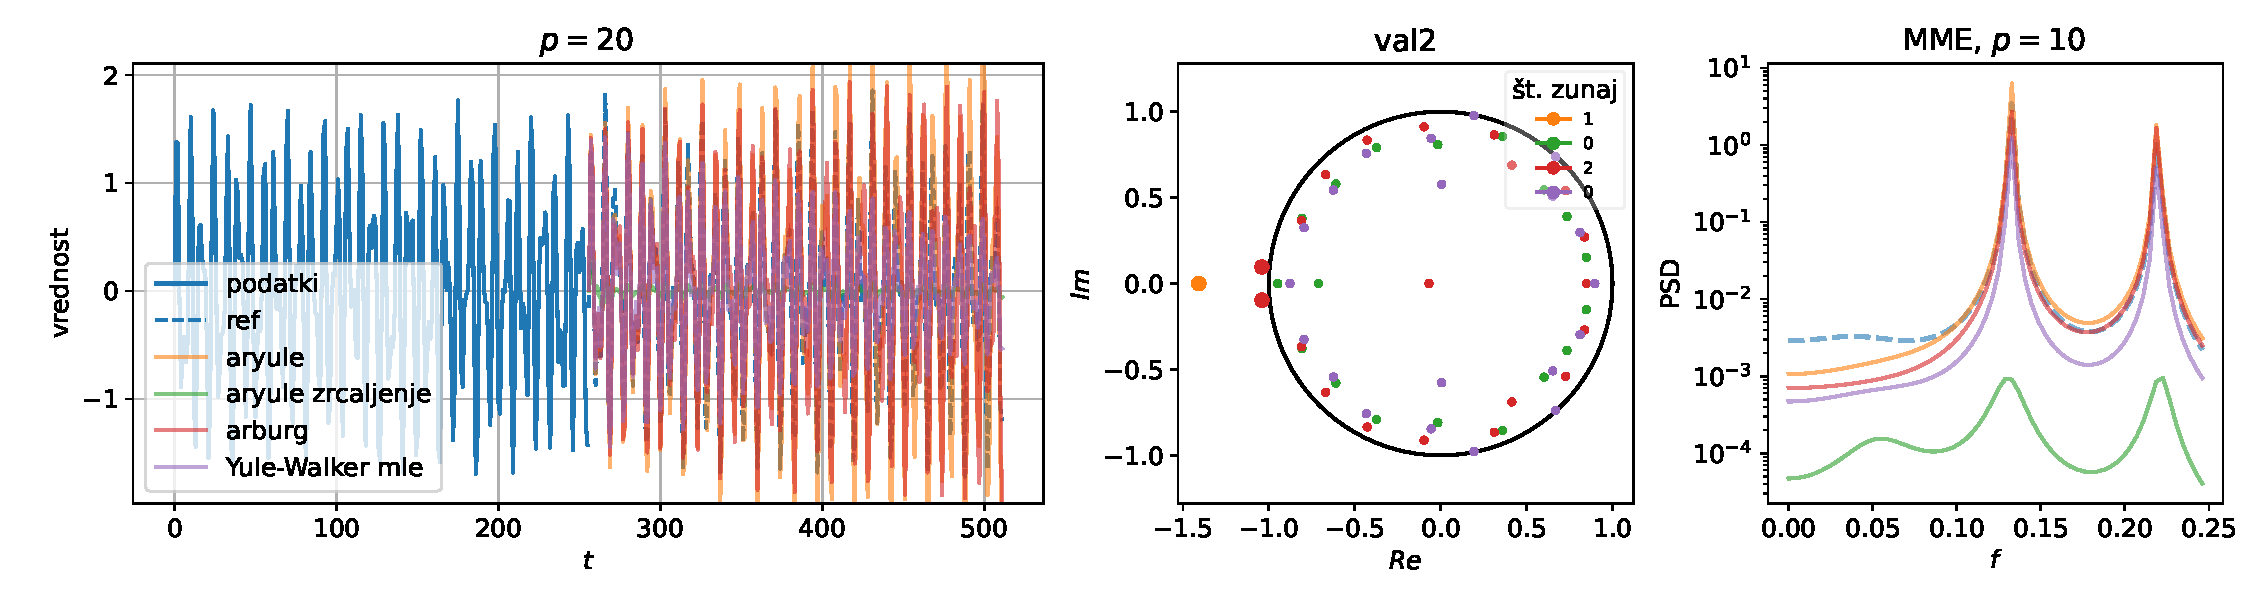
\includegraphics[width=\linewidth]{12.nal_slike/napoved_val2.pdf}
        \caption{}
    \end{subfigure}
    \begin{subfigure}{\textwidth}
        \centering
        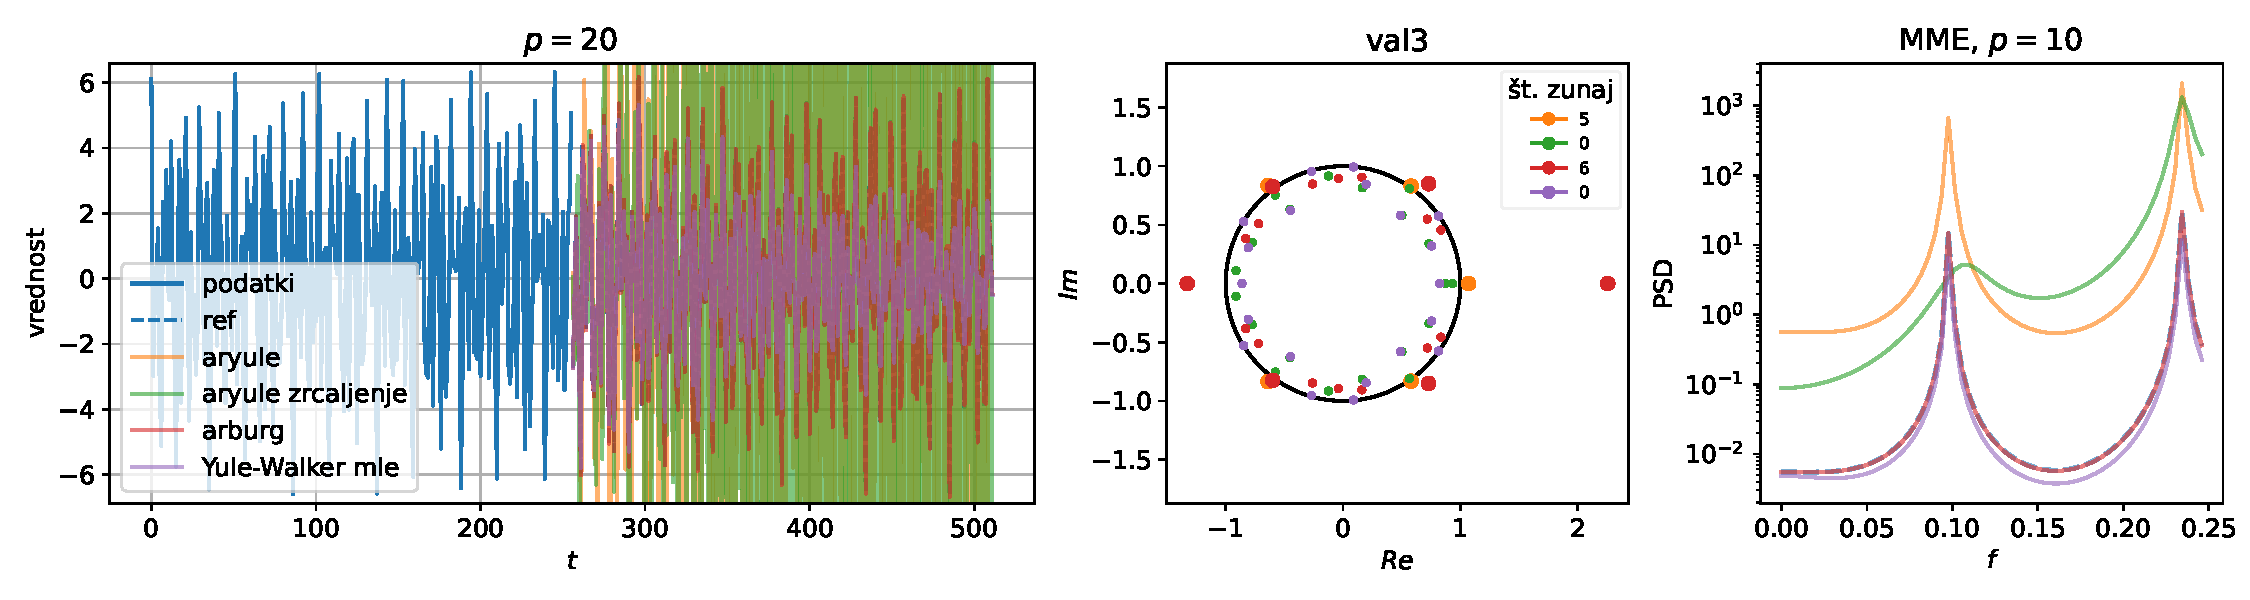
\includegraphics[width=\linewidth]{12.nal_slike/napoved_val3.pdf}
        \caption{}
    \end{subfigure}
    \begin{subfigure}{\textwidth}
        \centering
        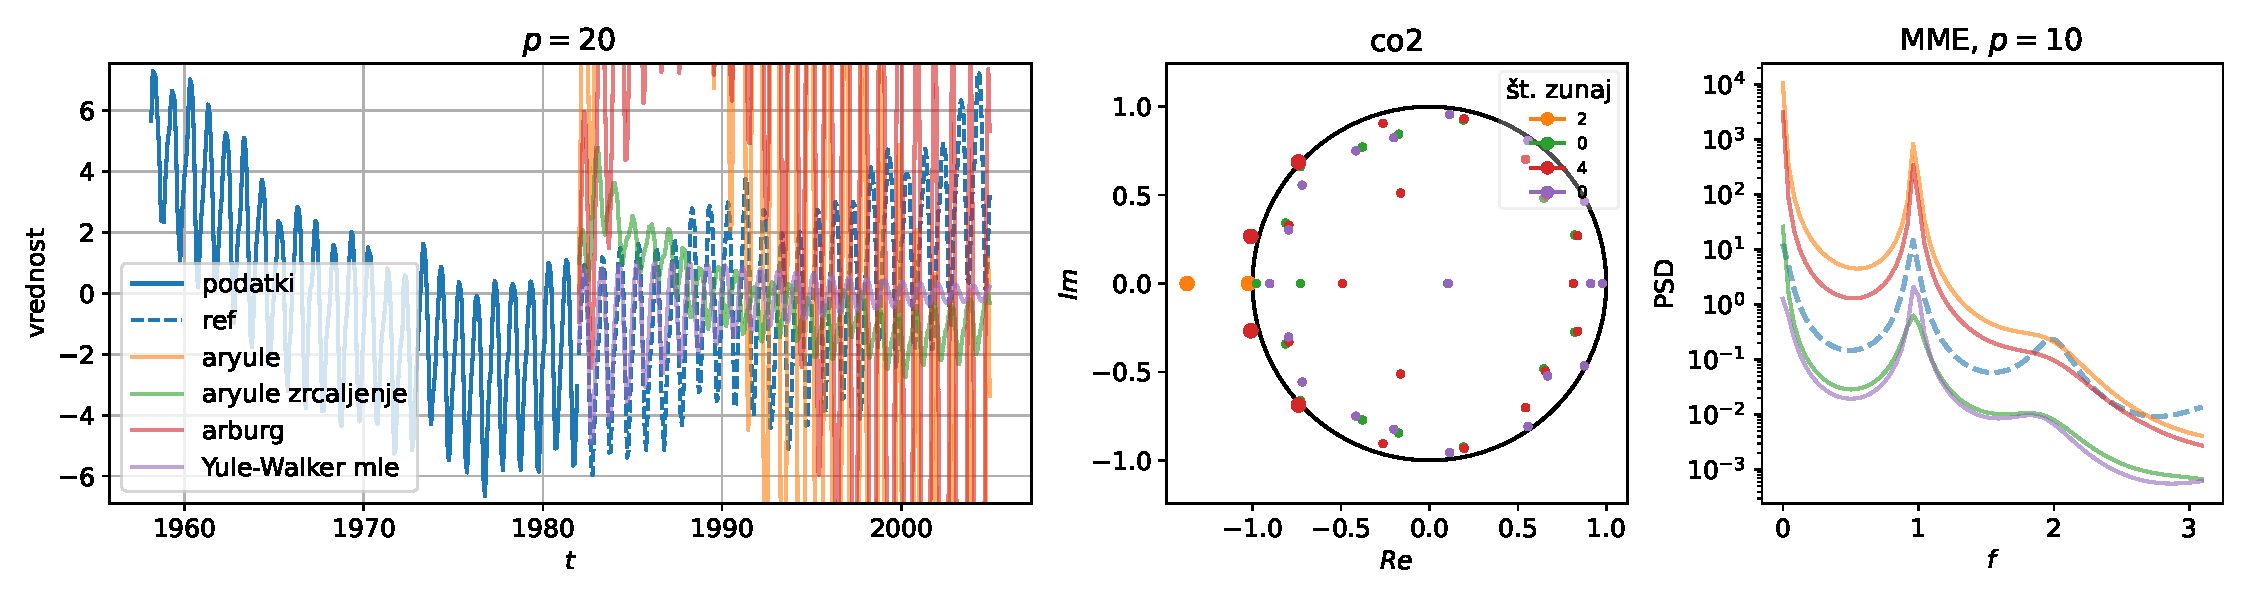
\includegraphics[width=\linewidth]{12.nal_slike/napoved_co2.pdf}
        \caption{}
    \end{subfigure}
    \caption[short]{Napoved za (a) val2.dat, (b) val3.dat in (c) co2.dat}
\end{figure}

Za lažjo predstavo uspešne nnapovedi, sem izračunal, kako se spreminja relativna napaka med napovedjo in referenco. Pri višjih redih se presenetljivo dobro obnese \texttt{AutoReg}, predvsem pri val3 lahko rečem, da popolnoma pralivno napove signal! Vendar ta funcija ne vrne podatka to koeficientih in posledično o polih. Ostale metode imajo podobno točnost kot pri val2. Ta primer je predstavljen na sliki \ref{fig:autoreg}. Najbolj problematičen signal za napoved je co2.

\begin{figure}[ht]
    \centering
    \begin{subfigure}{0.49\textwidth}
        \centering
        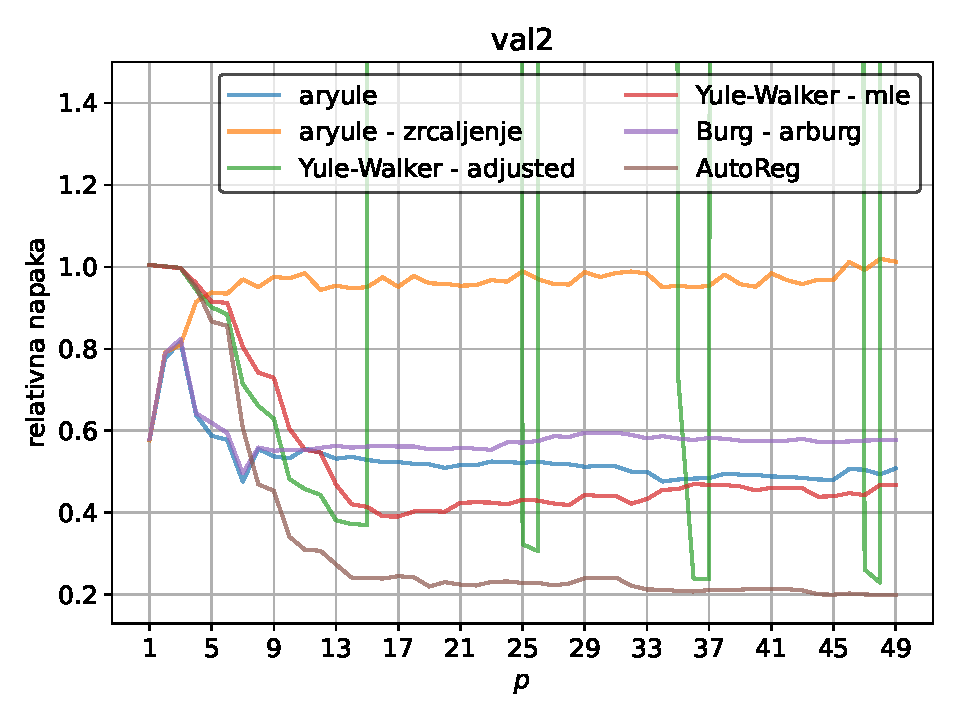
\includegraphics[width=\linewidth]{12.nal_slike/napaka_val2.pdf}
        \caption{}
    \end{subfigure}
    \begin{subfigure}{0.49\textwidth}
        \centering
        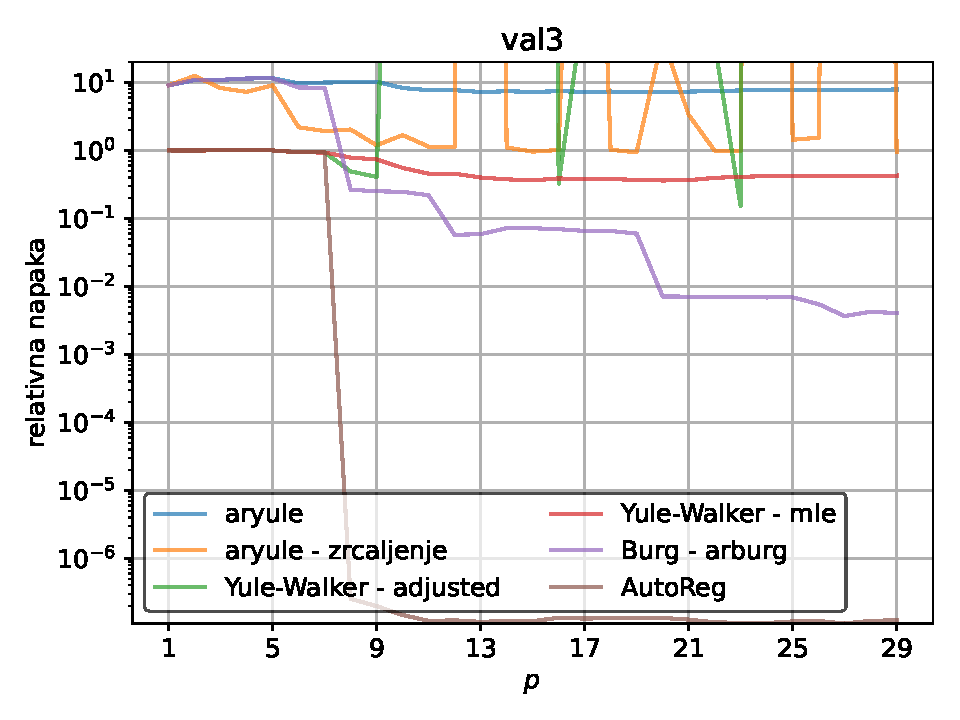
\includegraphics[width=\linewidth]{12.nal_slike/napaka_val3.pdf}
        \caption{}
    \end{subfigure}
    \begin{subfigure}{\textwidth}
        \centering
        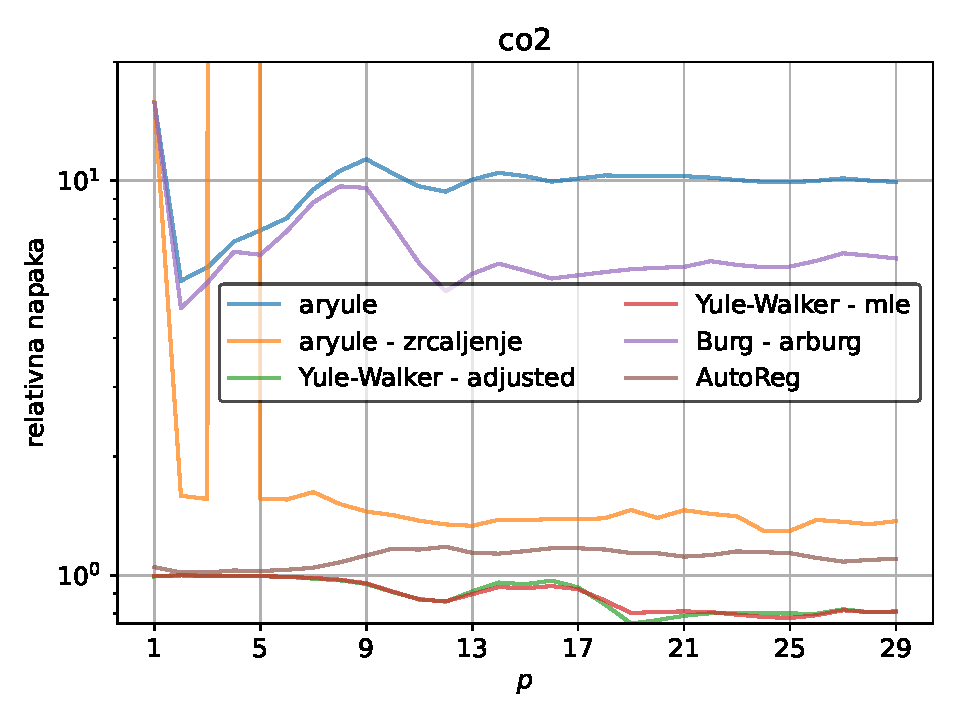
\includegraphics[width=0.5\linewidth]{12.nal_slike/napaka_co2.pdf}
        \caption{}
    \end{subfigure}
    \caption[short]{Napaka napovedi za (a) val2.dat, (b) val3.dat in (c) co2.dat}
\end{figure}

\begin{figure}[ht!]
    \centering
    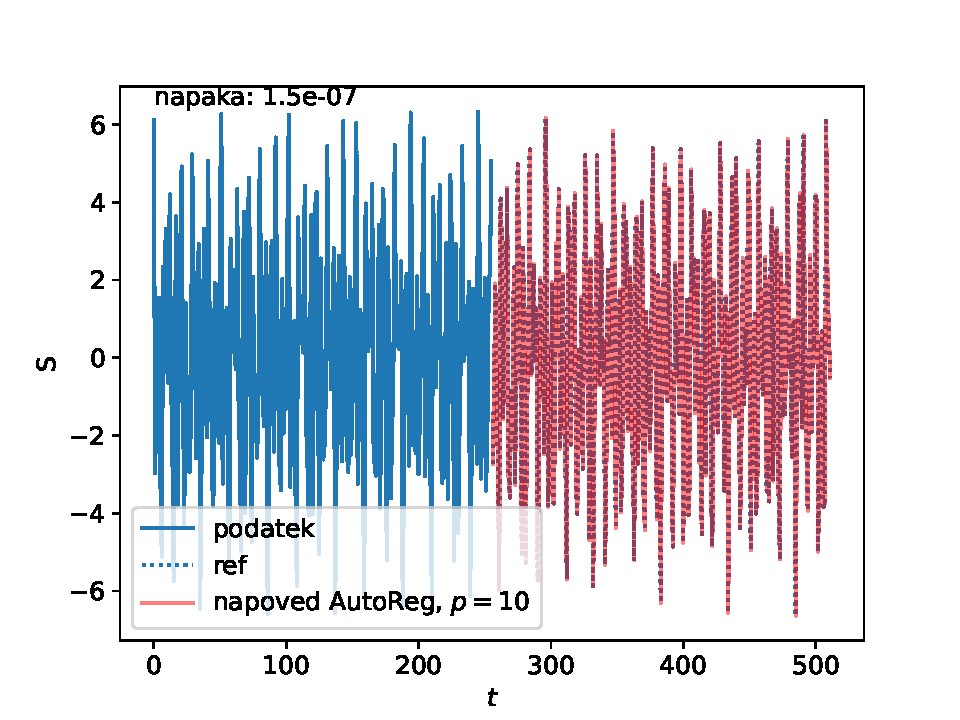
\includegraphics[width=0.65\linewidth]{12.nal_slike/napoved_val3_autoreg.pdf}
    \caption[short]{(Zelo dobra) napoved signala val3 z \texttt{statsmodels.tsa.ar\_model.AutoReg}}\label{fig:autoreg}
\end{figure}

\subsection{Signali iz druge naloge}

Na spodnji sliki so prikazani spektri PSD za celoten signal po metodi MME, zgolj zato, da se lahko pri napovedi primerjamo s tem. Opazimo lahko značilni periodi signala:
\begin{itemize}
    \item Lunine efemeride imajo periodo luninega meseca (cca 28 dni).
    \item Wolfovo število ima periodo števila sončevih peg (cca 11 let).
\end{itemize}
Borzni podatek ne pričakovano izkazuje periodike! V tem primeru PSD ni uporaben.

\begin{figure}[ht]
    \begin{subfigure}{0.49\textwidth}
        \centering
        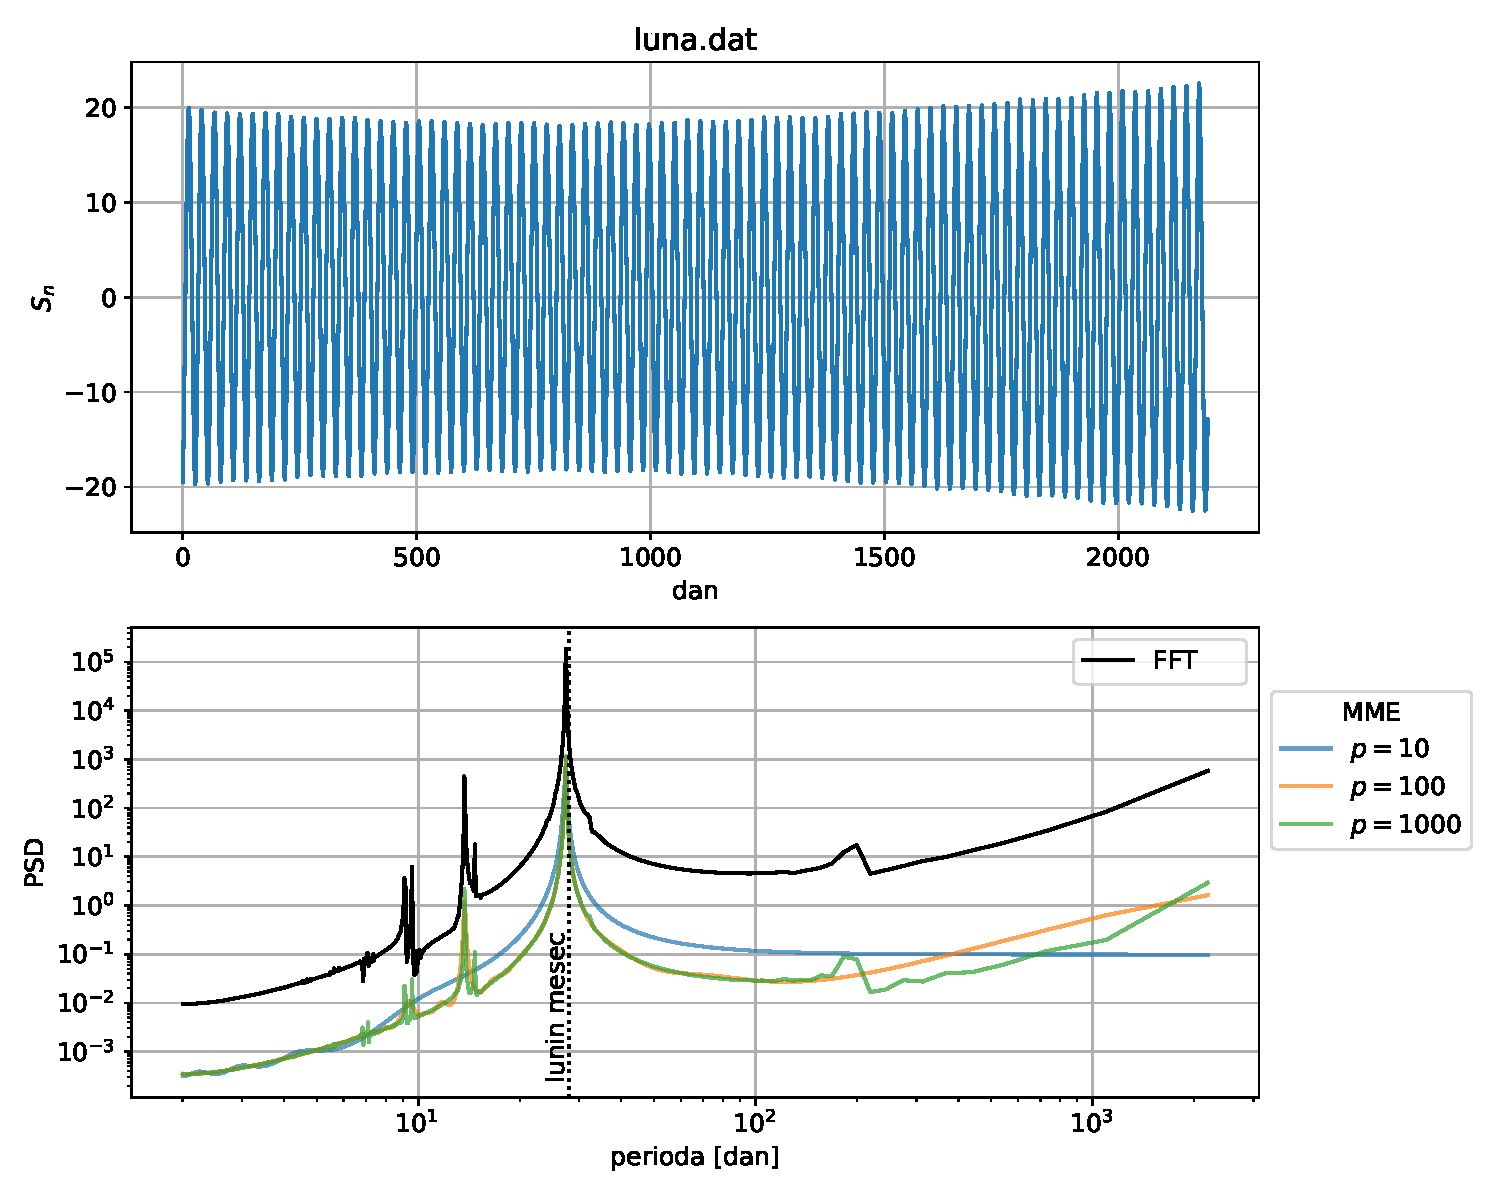
\includegraphics[width=\linewidth]{12.nal_slike/12.1/luna_PDS.pdf}
        \caption{}
    \end{subfigure}
    \begin{subfigure}{0.49\textwidth}
        \centering
        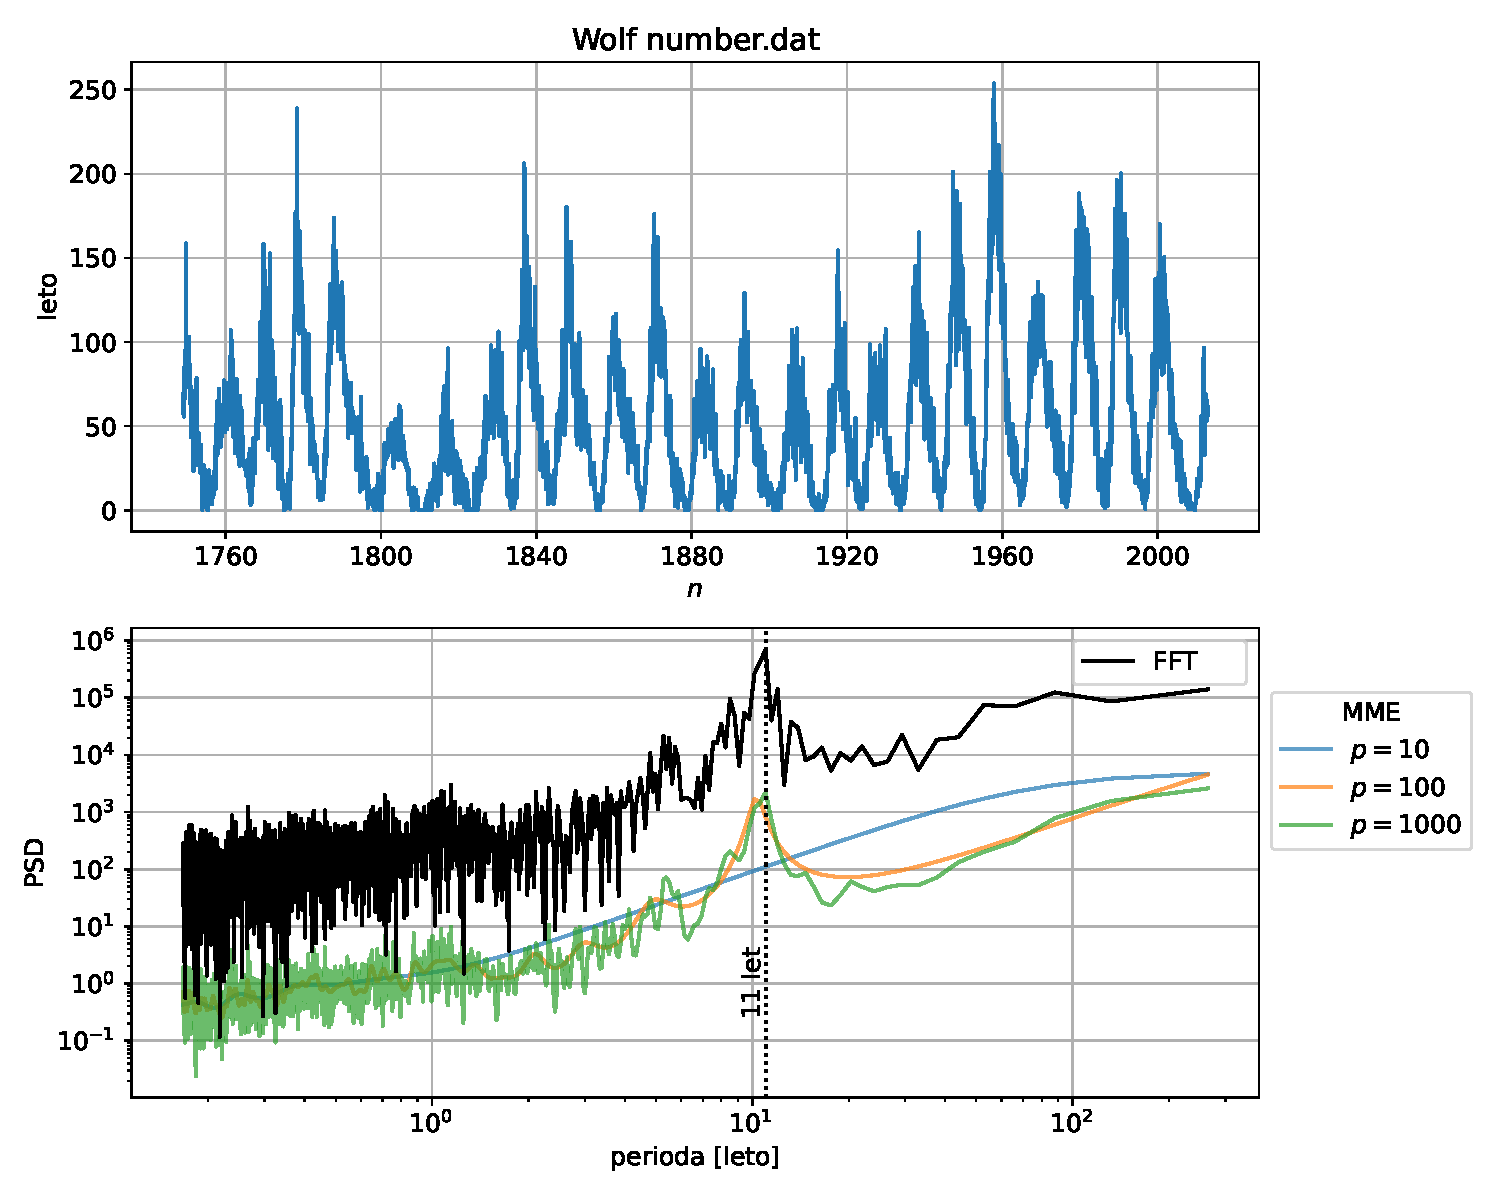
\includegraphics[width=\linewidth]{12.nal_slike/12.1/wolf_PSD.pdf}
        \caption{}
    \end{subfigure}
    \begin{subfigure}{\textwidth}
        \centering
        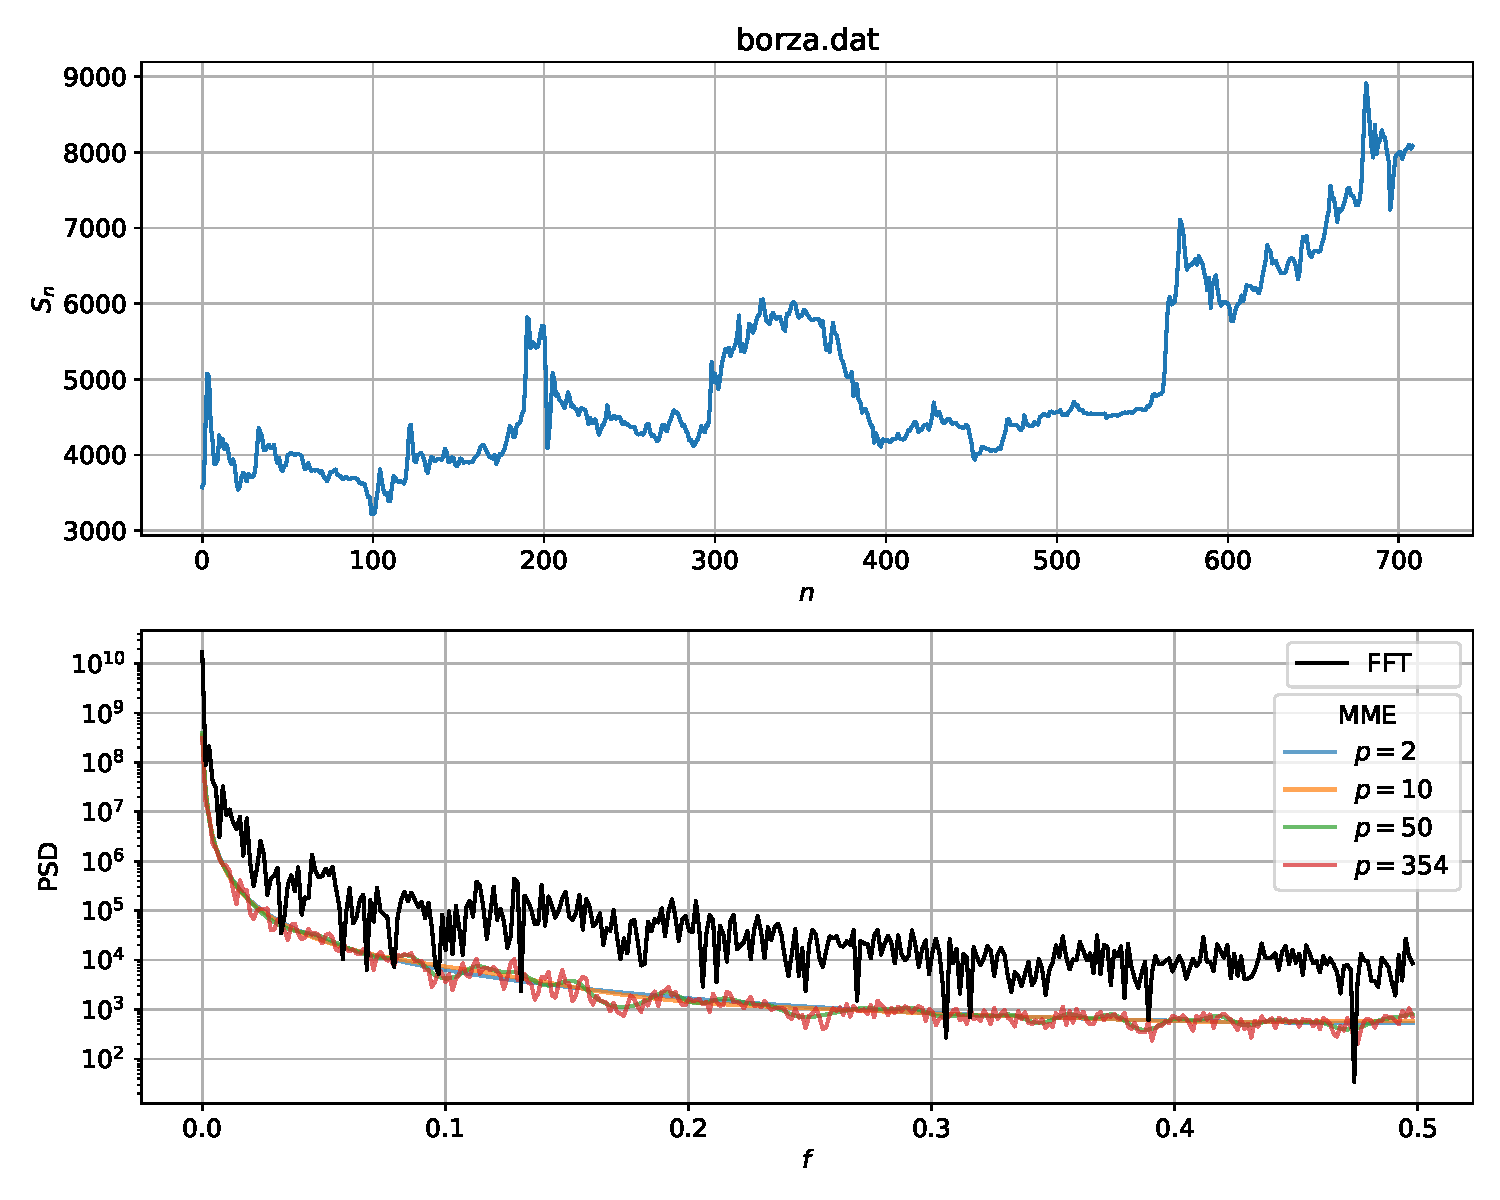
\includegraphics[width=0.5\linewidth]{12.nal_slike/12.1/borza_PSD.pdf}
        \caption{}
    \end{subfigure}
    \caption[short]{PSD (a) luninih efemerid, (b) Wolfovega števila in (c) borznega podatka}
\end{figure}

Sedaj se lotimo napovedi podatkov, tako kot v prejšnjem podpoglavju. Rezultati so vidni na spodnji sliki. Skupaj z določitvijo relativne napake napovedi glede na referenco, kot smo to storili že poprej in analizo spektra lahko ugotovimo pravilnost napovedi tako amplitudno, kot tudi fazno! Zavoljo preglednosti nisem prikazoval vseh metod, vendar le najbolj uspešne. Opomba: \texttt{AutoReg} tukaj nisem poizkušal!

Opazim, da ne obstaja univerzalno najboljša metoda. V splošnem se še najbolje obnese Yule-walker z maximum-likehood estimation. Presenetljivo pa je, da je pri luni algoritem Burg očitno boljši, čeprav so 3 poli izven enotkega kroga. 

Pri Wolfu je potrebno povečati število polov, da sploh ujamemo periodo, amplituda pa sicer zelo hitro pade. Povečevanje polov ne pomaga, pojavijo se neželene oscilacije! 

Predvsem pri borzi ima sicer napoved pravilen trend v začetku, nato pa se popolnoma izgubi. Višanje reda ne pomaga preveč. Podoben tred je opazen, tudi če zamaknemo mejo napovedi, kar pa je v primeru, prikazanem na spodnji sliki povsem neustrezno.

\begin{figure}[H]
    \begin{subfigure}{\textwidth}
        \centering
        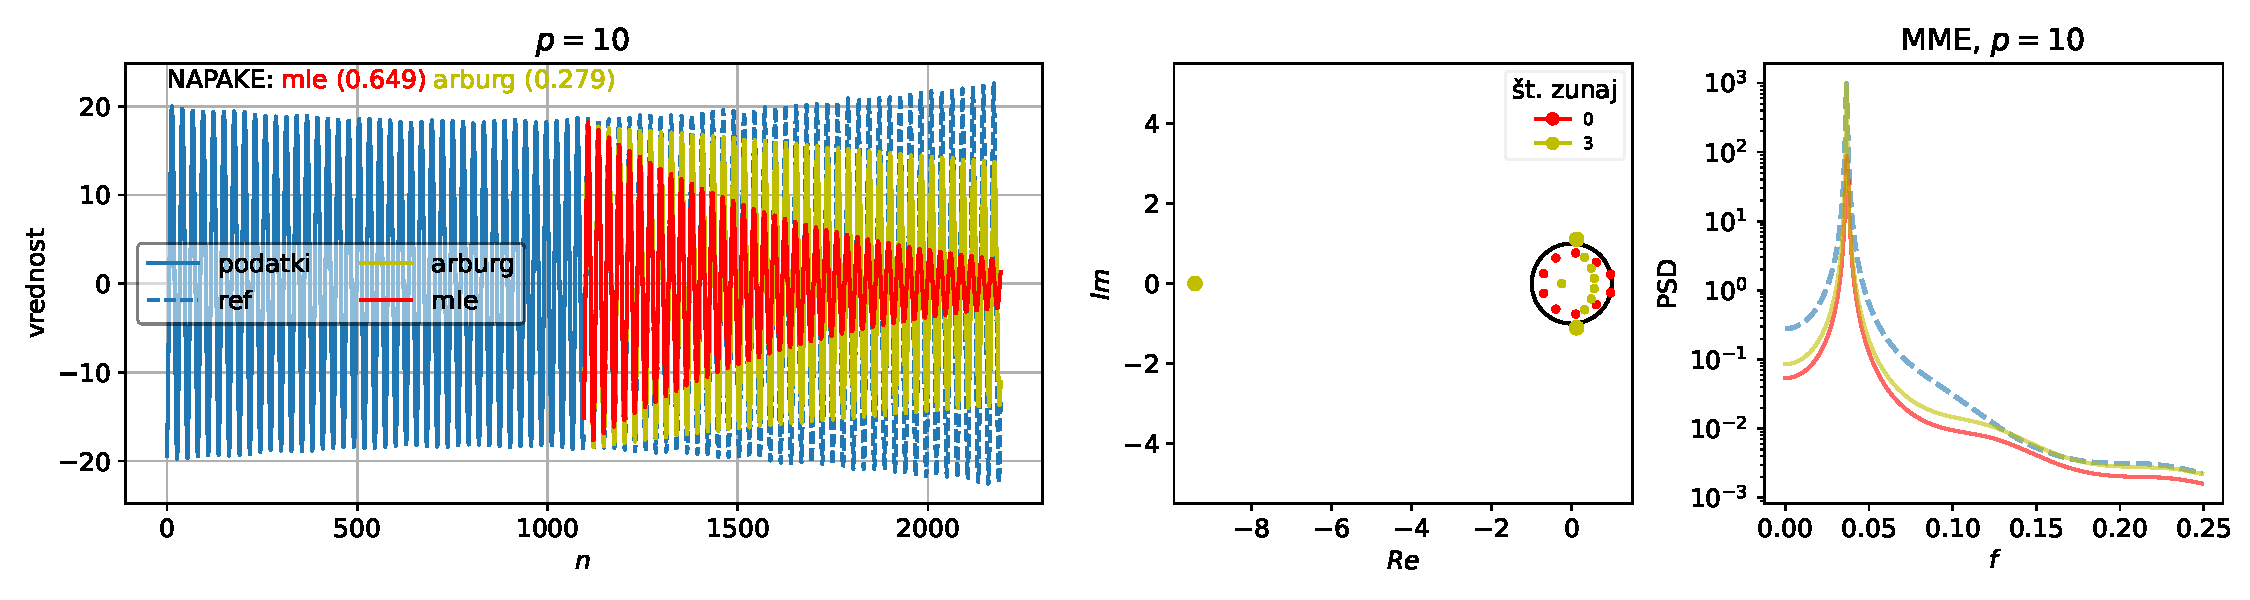
\includegraphics[width=\linewidth]{12.nal_slike/napoved_luna.pdf}
        \caption{}
    \end{subfigure}
    \begin{subfigure}{\textwidth}
        \centering
        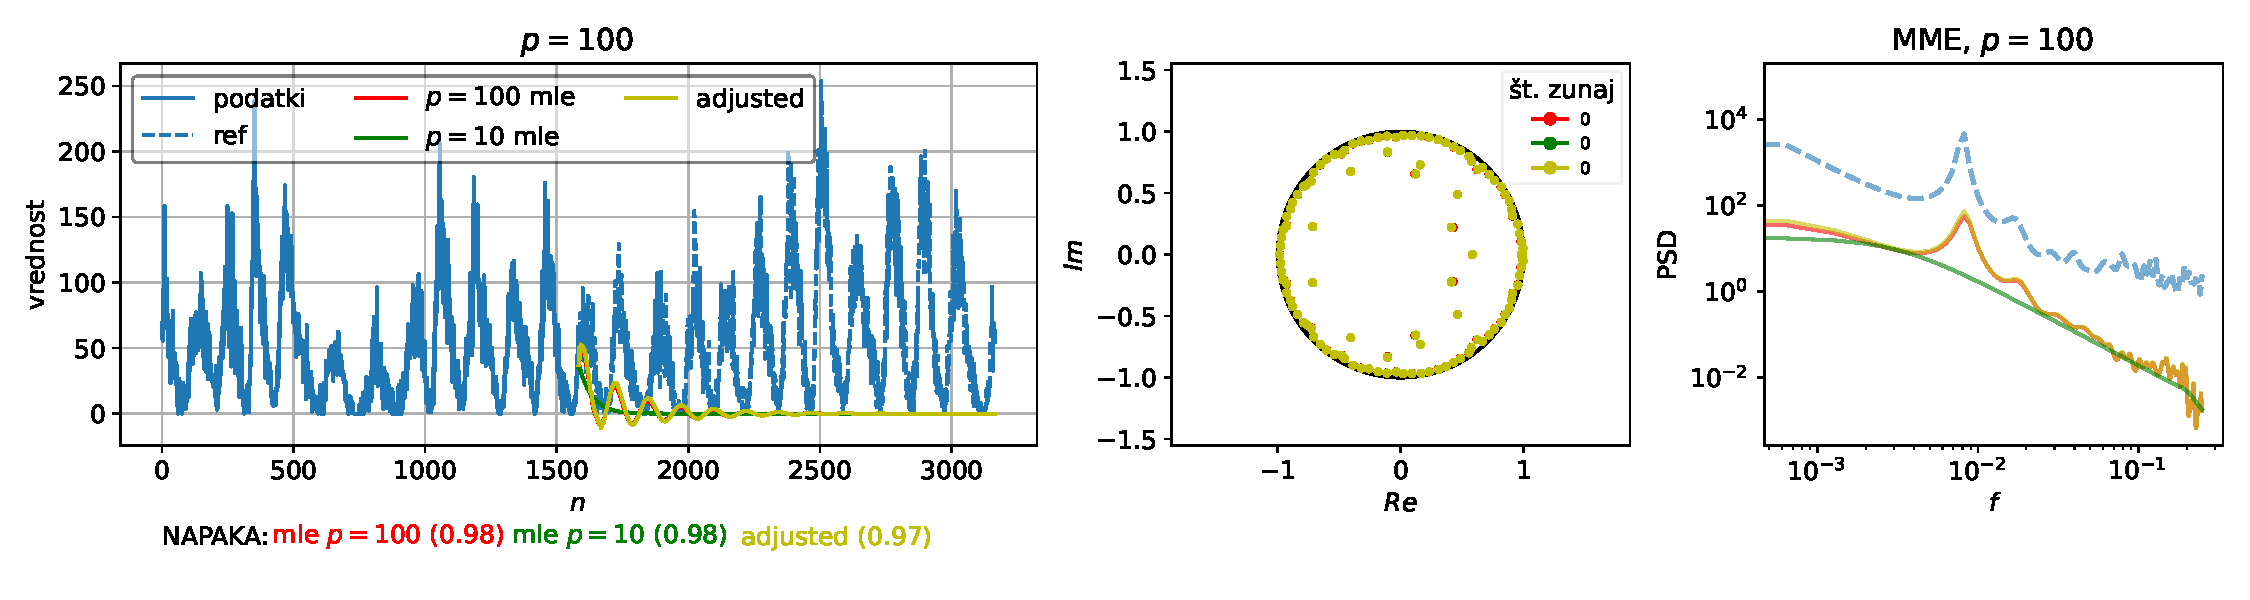
\includegraphics[width=\linewidth]{12.nal_slike/napoved_wolf.pdf}
        \caption{}
    \end{subfigure}
    \begin{subfigure}{0.75\textwidth}
        \centering
        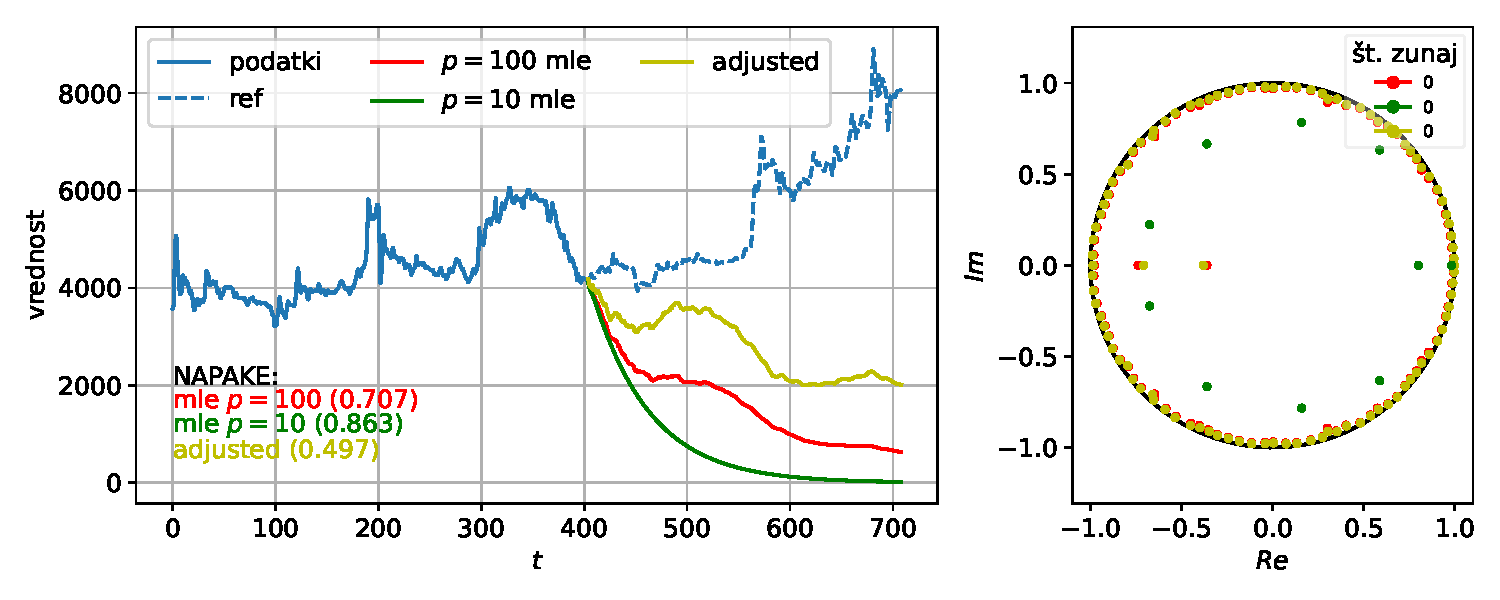
\includegraphics[width=\linewidth]{12.nal_slike/napoved_borza.pdf}
        \caption{}
    \end{subfigure}
    \begin{subfigure}{0.75\textwidth}
        \centering
        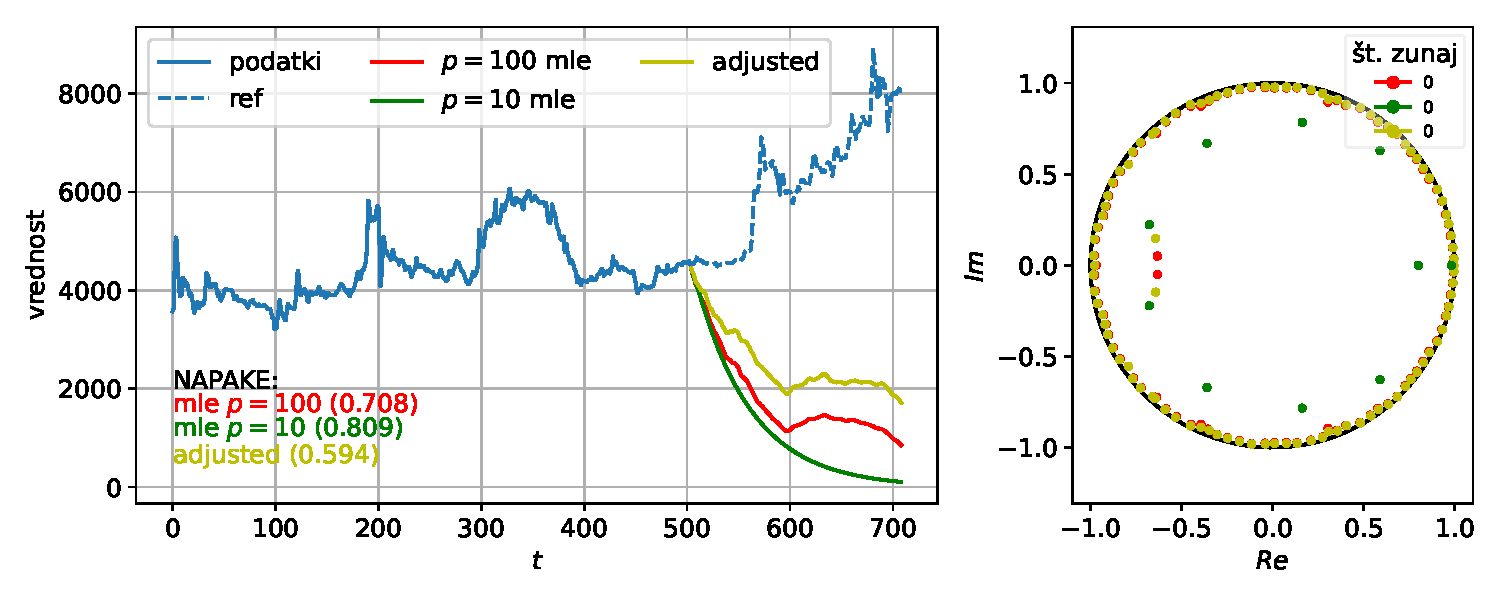
\includegraphics[width=\linewidth]{12.nal_slike/napoved_borza_zamik.pdf}
        \caption{}
    \end{subfigure}
    \caption[short]{Napoved (a) luninih efemerid, (b) Wolfovega števila, (c) borznega podatka in (d) zamik napovedi za 150 pri borzi}
\end{figure}

\newpage
\subsection{Vpliv šuma}

Poiskusimo tudi napovedati podatke, ki vsebujejo šum. Izvedem preizkus na testnem sinusu in ugotovim, da se MME odziva enako kot FFT. Šum je kmalu tako močan, da preglasi signal.

\begin{figure}[ht!]
    \centering
    \begin{subfigure}{0.49\linewidth}
        \centering
        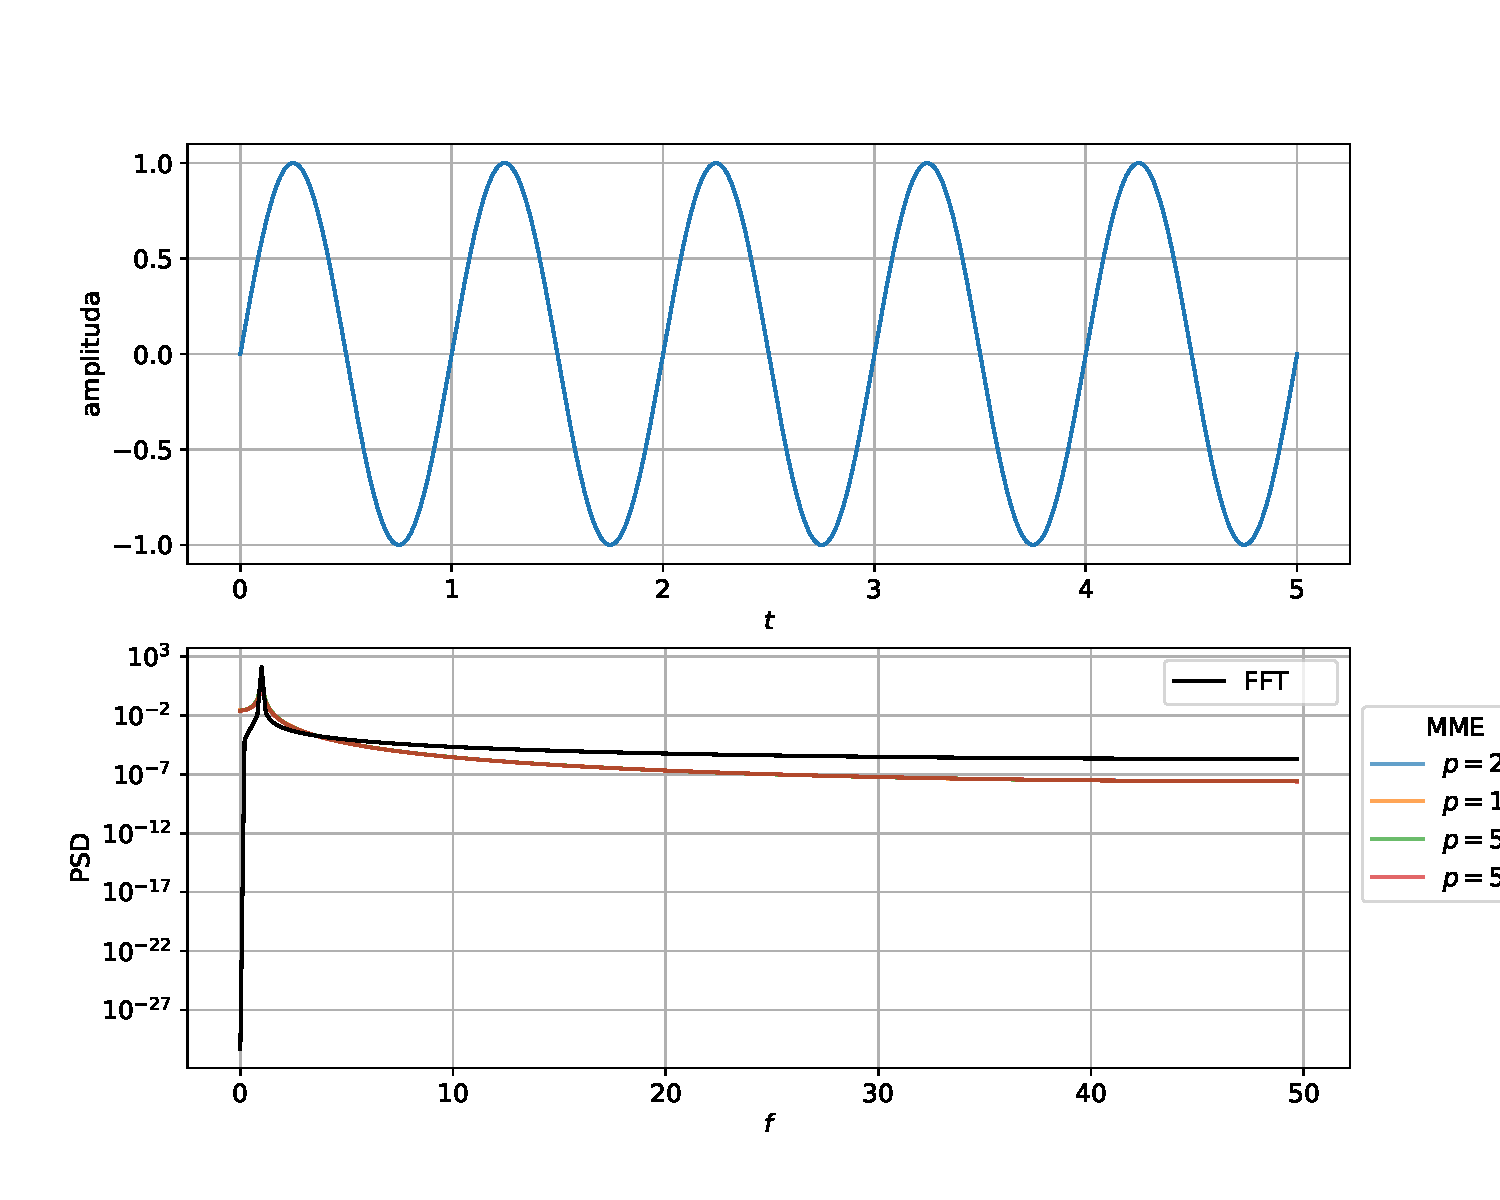
\includegraphics[width=\linewidth]{12.nal_slike/12.1/test_sin_rms0.pdf}
        \caption{}
    \end{subfigure}
    \begin{subfigure}{0.49\linewidth}
        \centering
        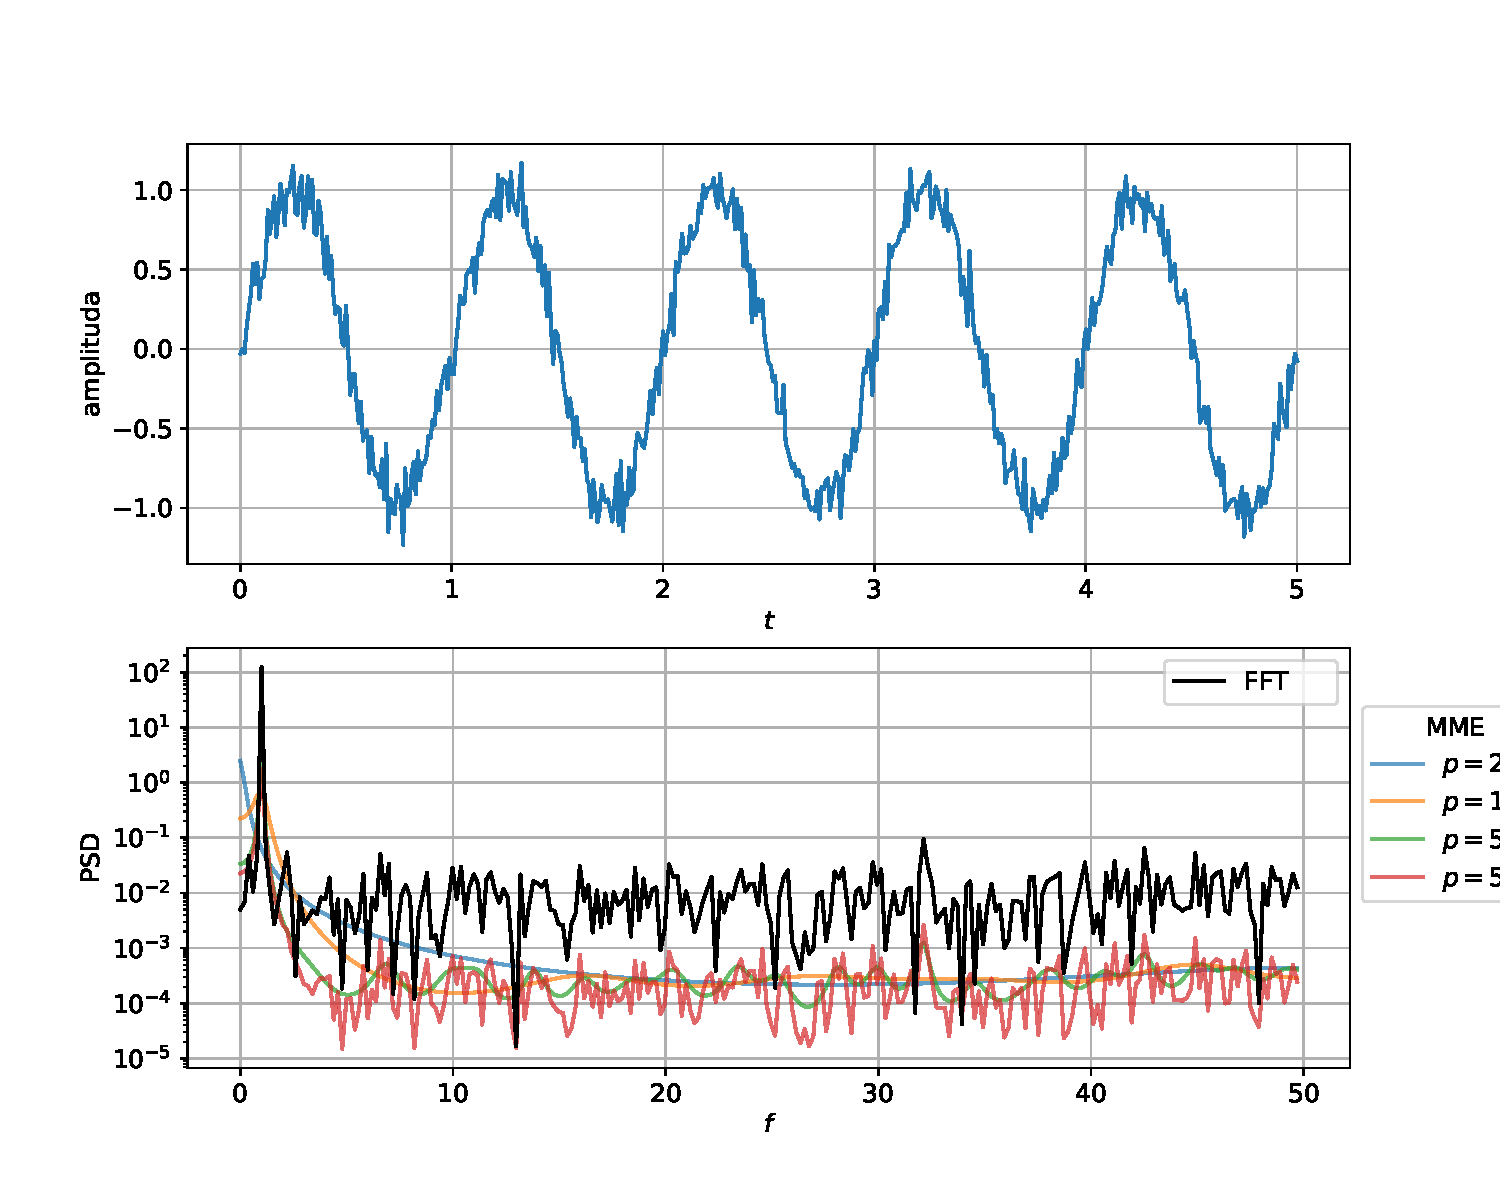
\includegraphics[width=\linewidth]{12.nal_slike/12.1/test_sin_rms0.1.pdf}
        \caption{}
    \end{subfigure}
    \begin{subfigure}{0.49\linewidth}
        \centering
        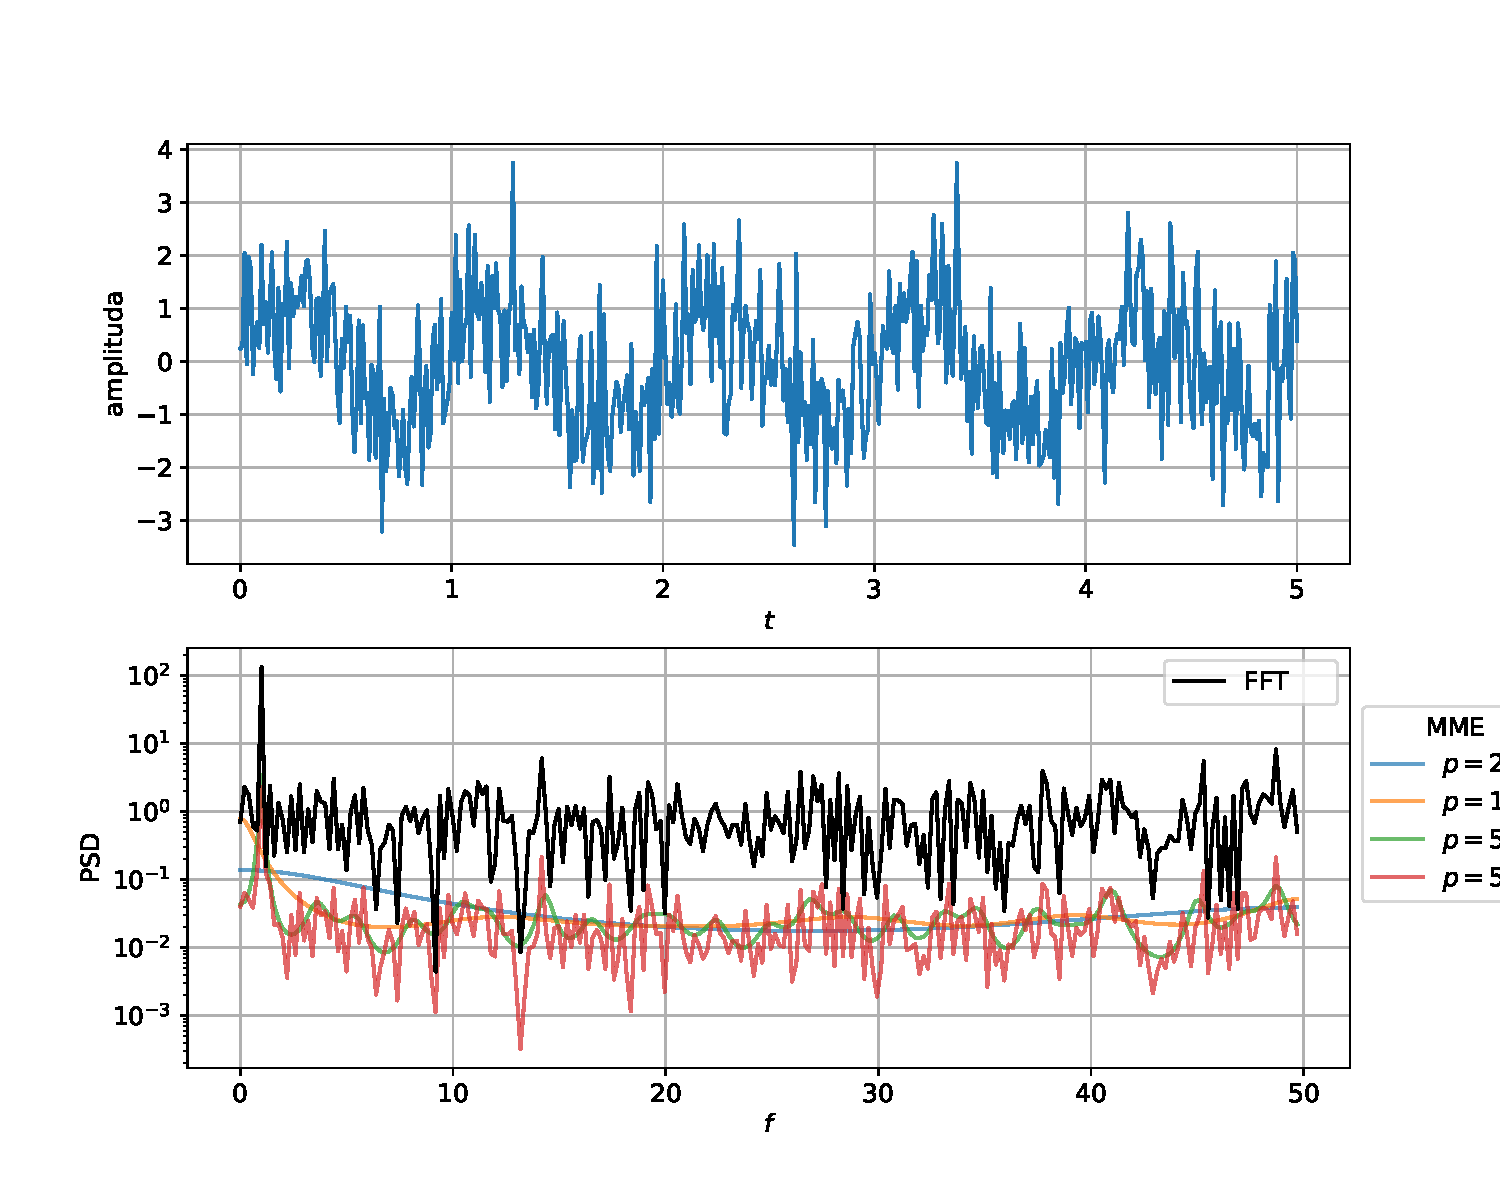
\includegraphics[width=\linewidth]{12.nal_slike/12.1/test_sin_rms1.pdf}
        \caption{}
    \end{subfigure}
    \begin{subfigure}{0.49\linewidth}
        \centering
        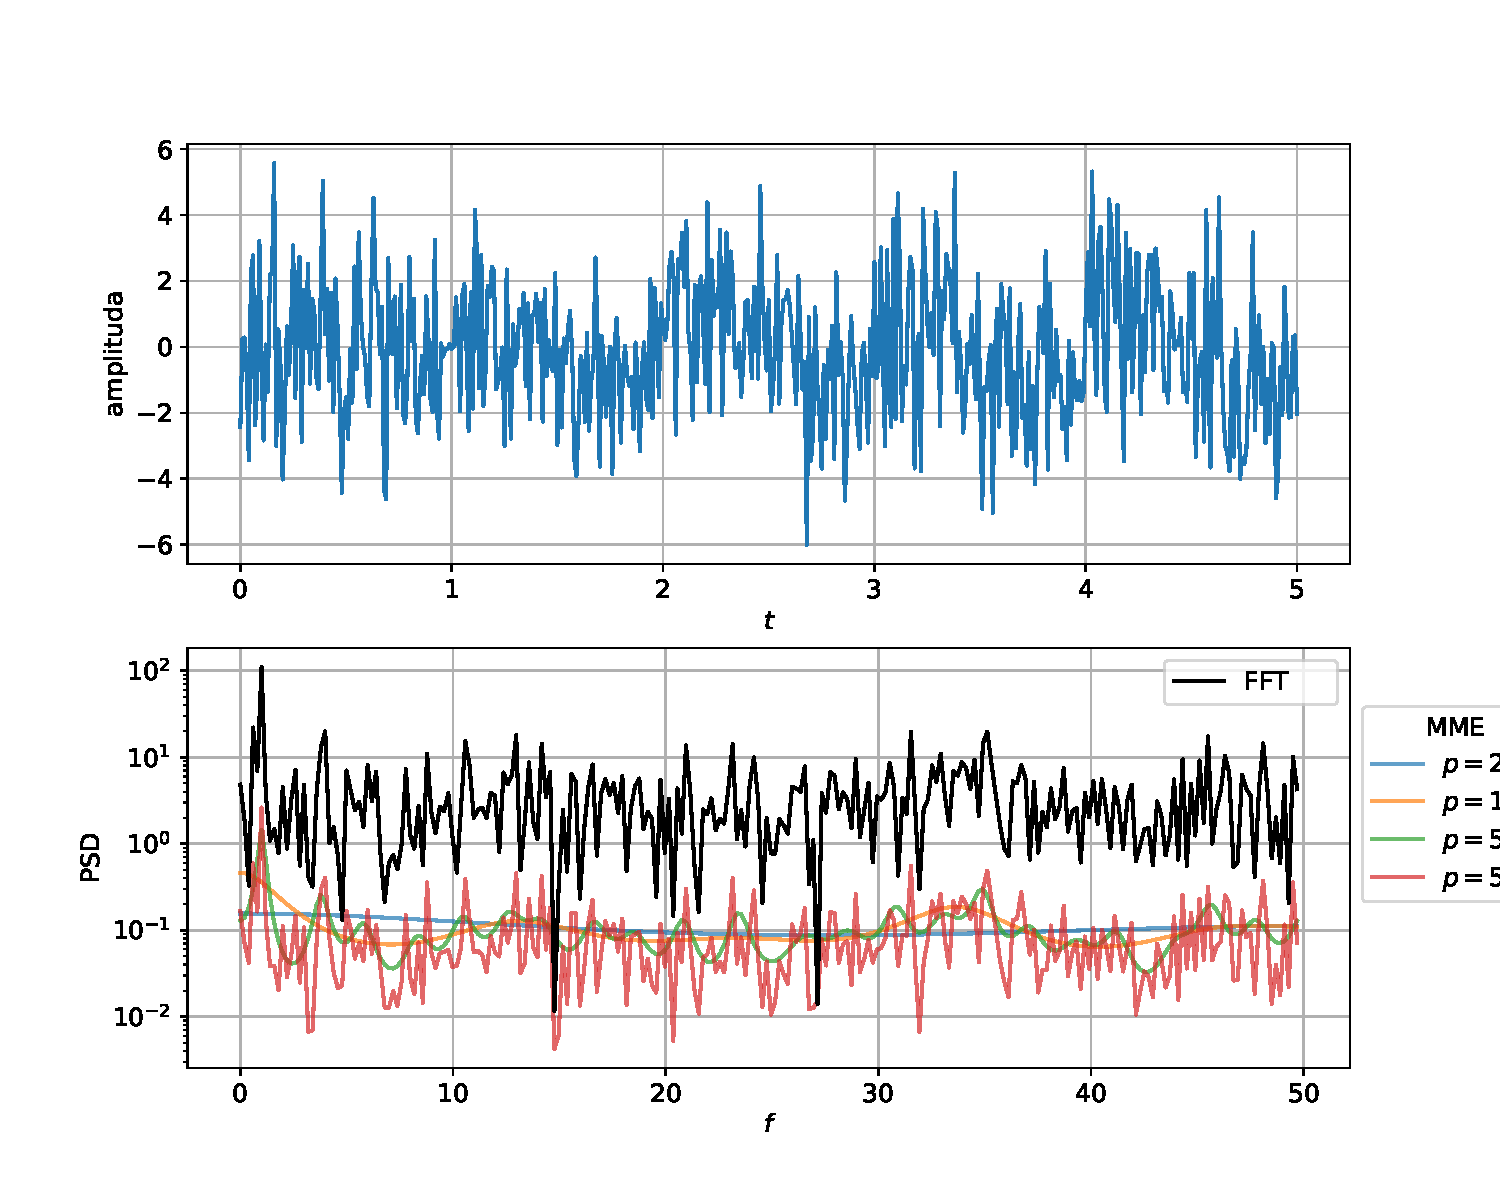
\includegraphics[width=\linewidth]{12.nal_slike/12.1/test_sin_rms2.pdf}
        \caption{}
    \end{subfigure}
    \caption[short]{RMS šuma na testnem sinusu (a) brez, (b) 0.1, (c) 1 in (d) 2}
\end{figure}

Ko poizkušam z napovednjo nad takim signalom, ta kmalu odpove. Pri relativno nizkem šumu sicer še ujame frekvenco, pri več pa nič več! Presenetljivo je, da se na spektru bolje ohranijo frekvence pri signalu val3, kot pri sinusu, verjetno zato, ker je amplituda večja. Amplituda napovedi se močno poveča, zato napake v tem primeru sploh ni smiselno računati. Tako zvano dušenje je tudi večje; amplituda z večanjem šuma hitreje pada in celo popolnoma preneha nihati ali pa se vedno bolj povečuje.

\begin{figure}[ht!]
    \centering
    \begin{subfigure}{\linewidth}
        \centering
        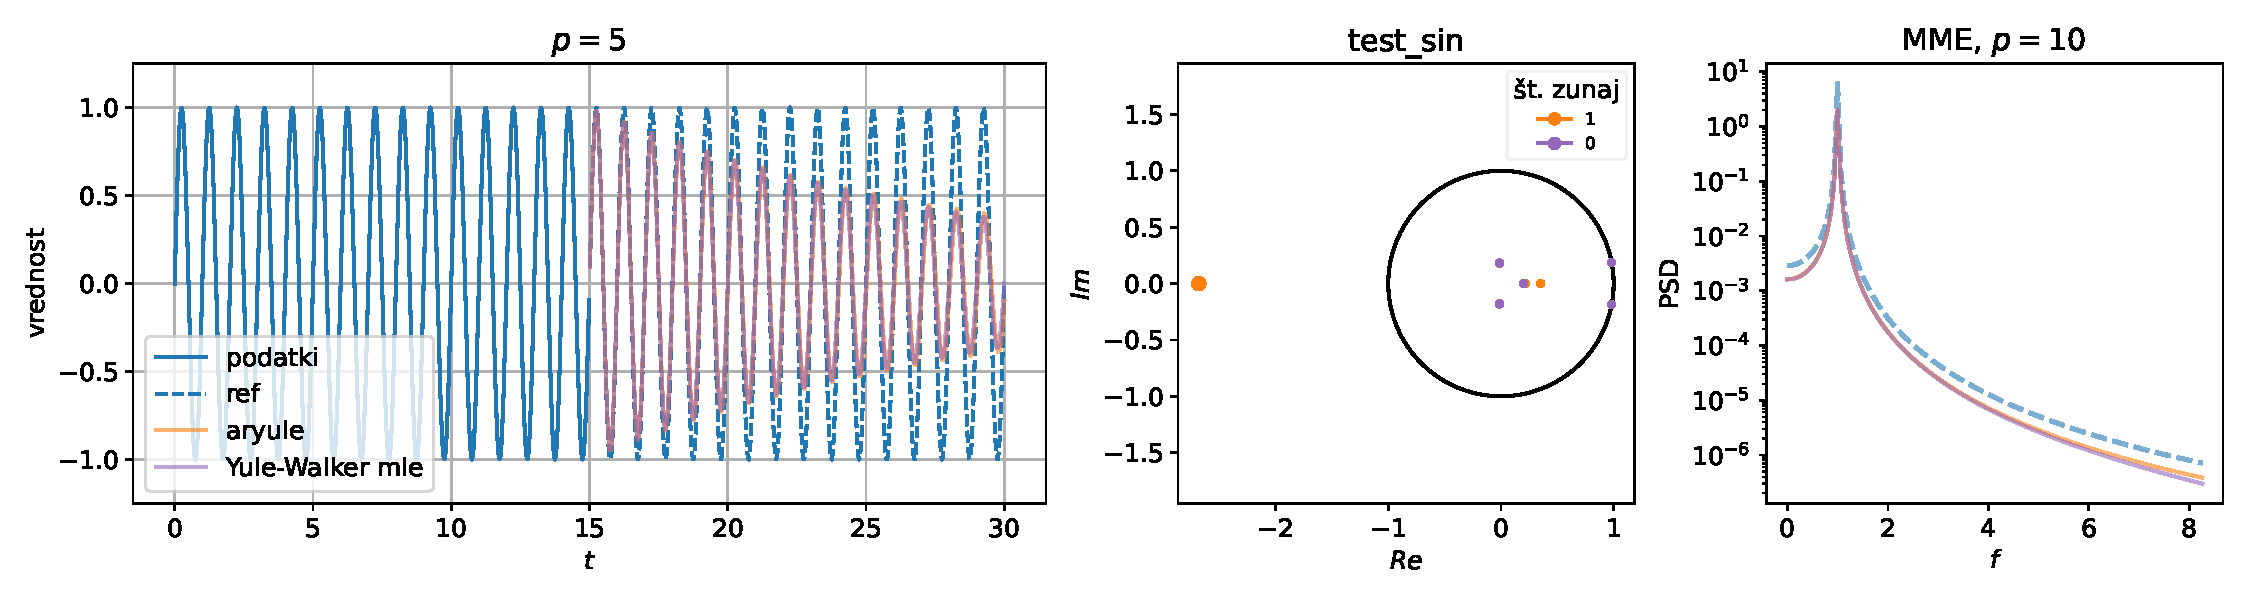
\includegraphics[width=\linewidth]{12.nal_slike/test_sin_šum0.pdf}
        \caption{}
    \end{subfigure}
    \begin{subfigure}{\linewidth}
        \centering
        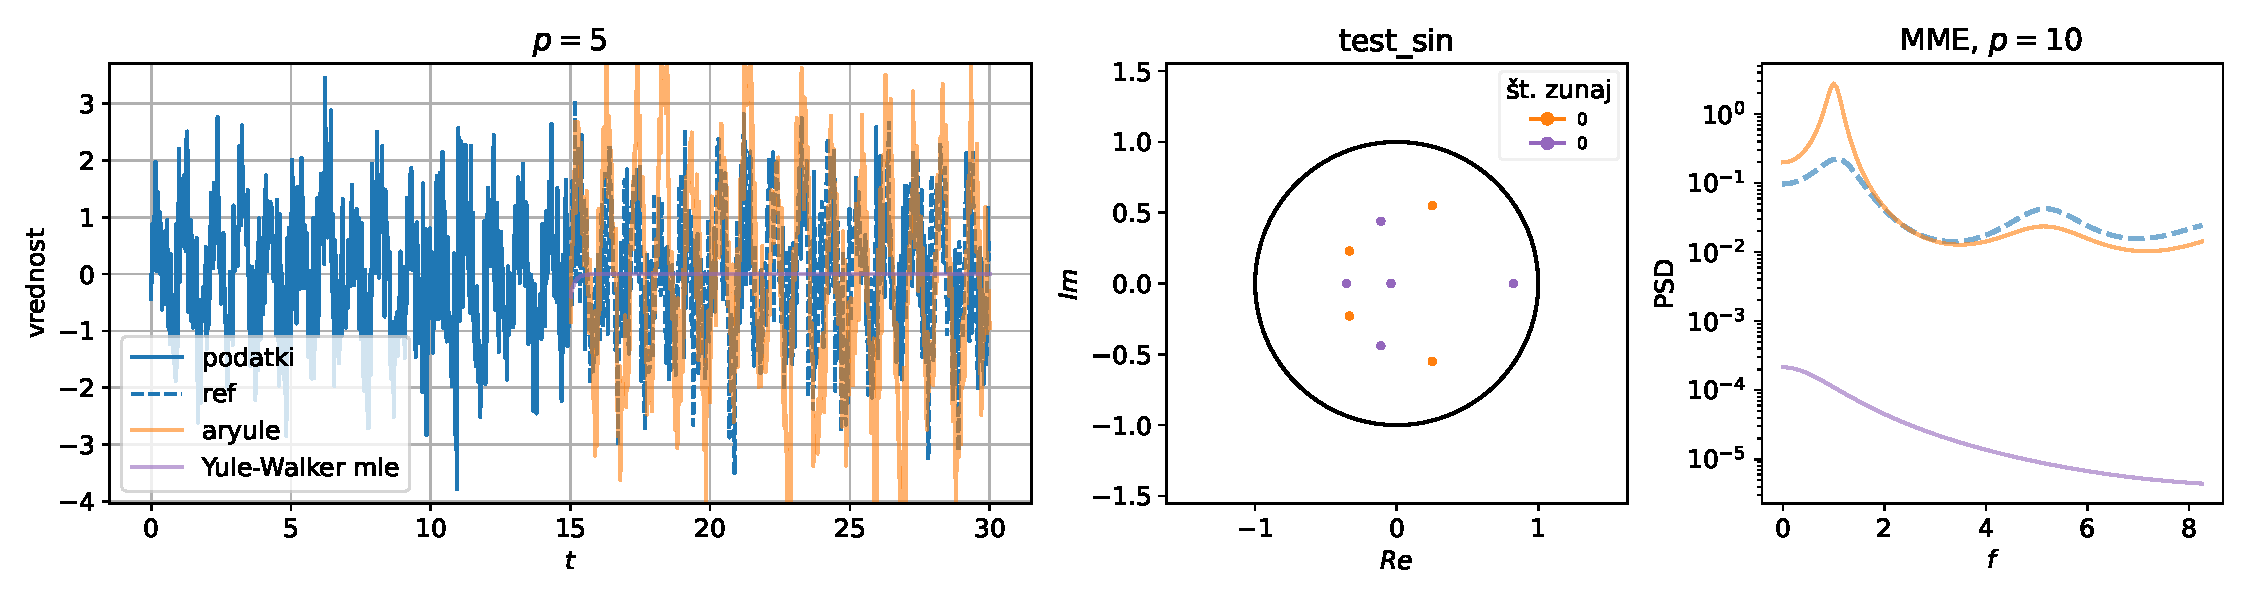
\includegraphics[width=\linewidth]{12.nal_slike/test_sin_šum1.pdf}
        \caption{}
    \end{subfigure}
    \caption[short]{Napoved zašumjenih podatkov testnega sinusa (a) brez in (b) z RMS = 1 šuma}
\end{figure}

\begin{figure}[H]
    \centering
    \begin{subfigure}{\linewidth}
        \centering
        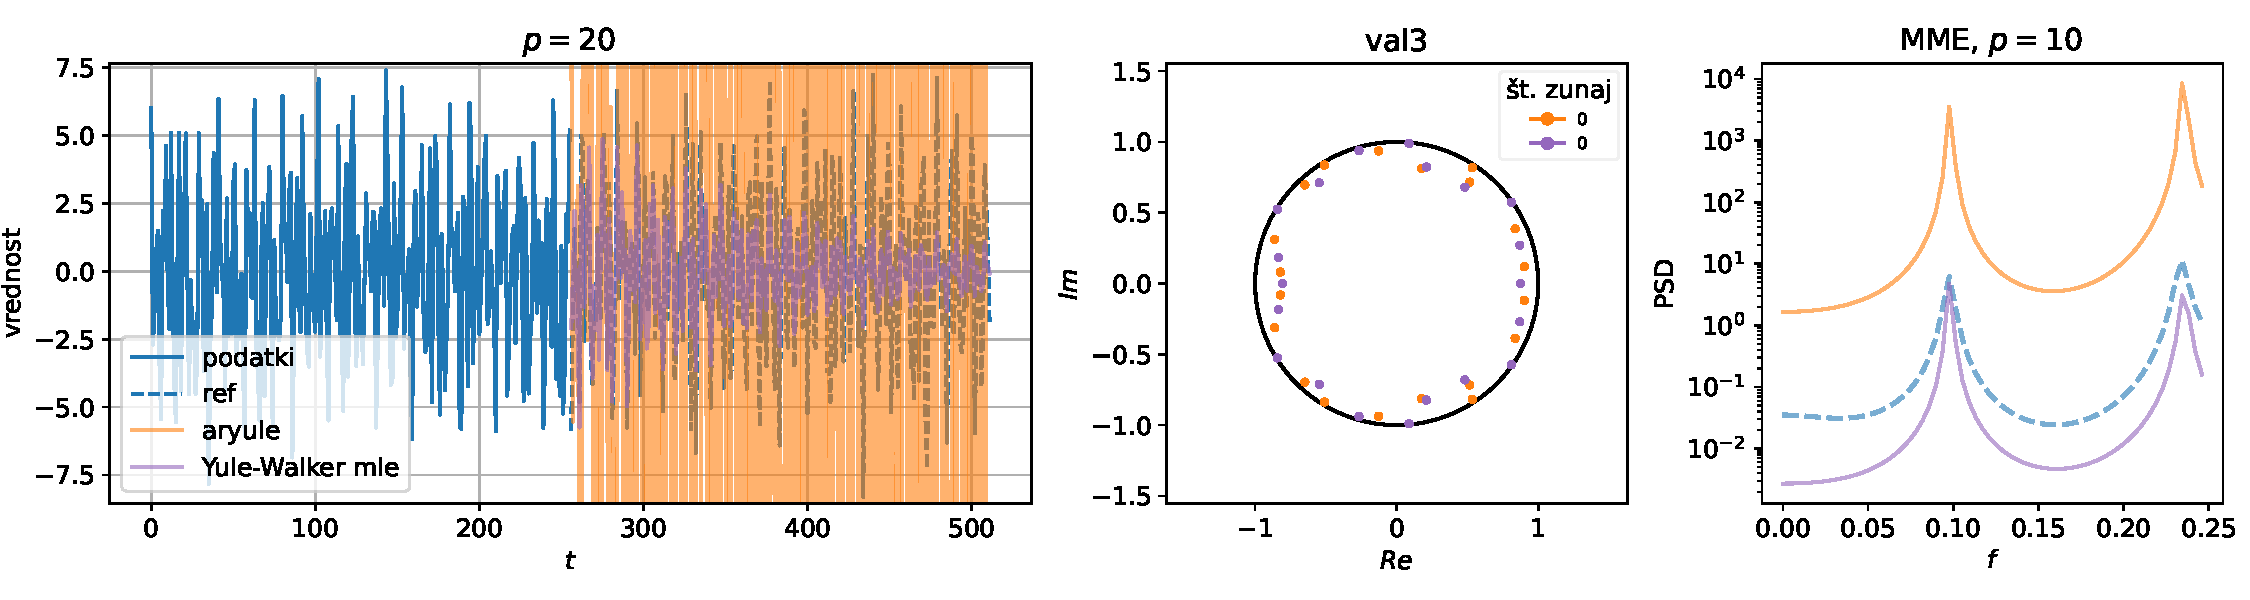
\includegraphics[width=\linewidth]{12.nal_slike/val3_šum1.pdf}
        \caption{}
    \end{subfigure}
    \begin{subfigure}{\linewidth}
        \centering
        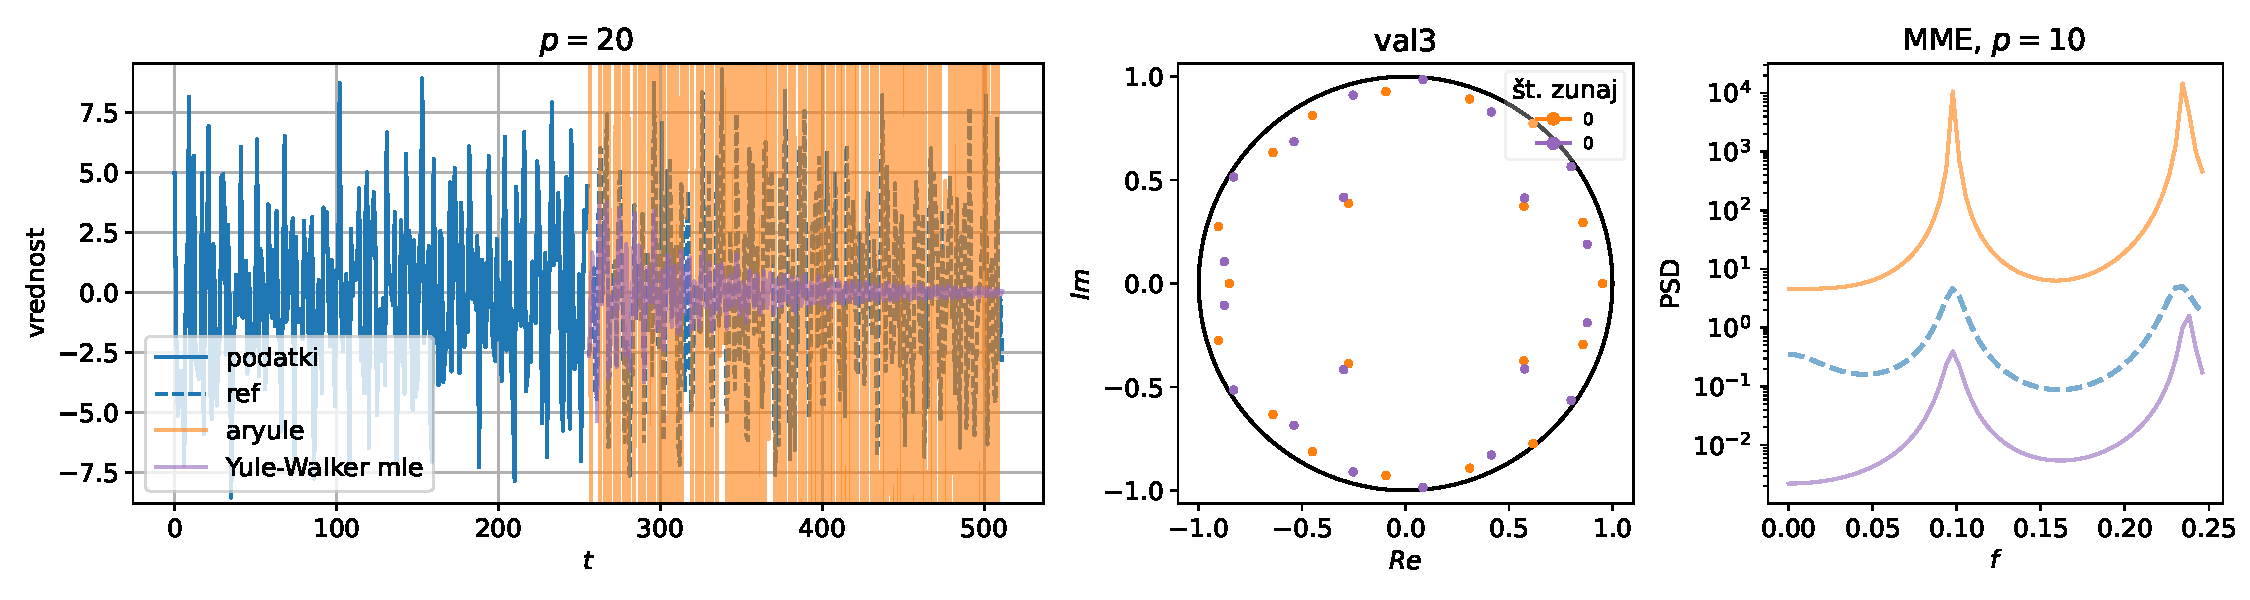
\includegraphics[width=\linewidth]{12.nal_slike/val3_šum2.pdf}
        \caption{}
    \end{subfigure}
    \begin{subfigure}{\linewidth}
        \centering
        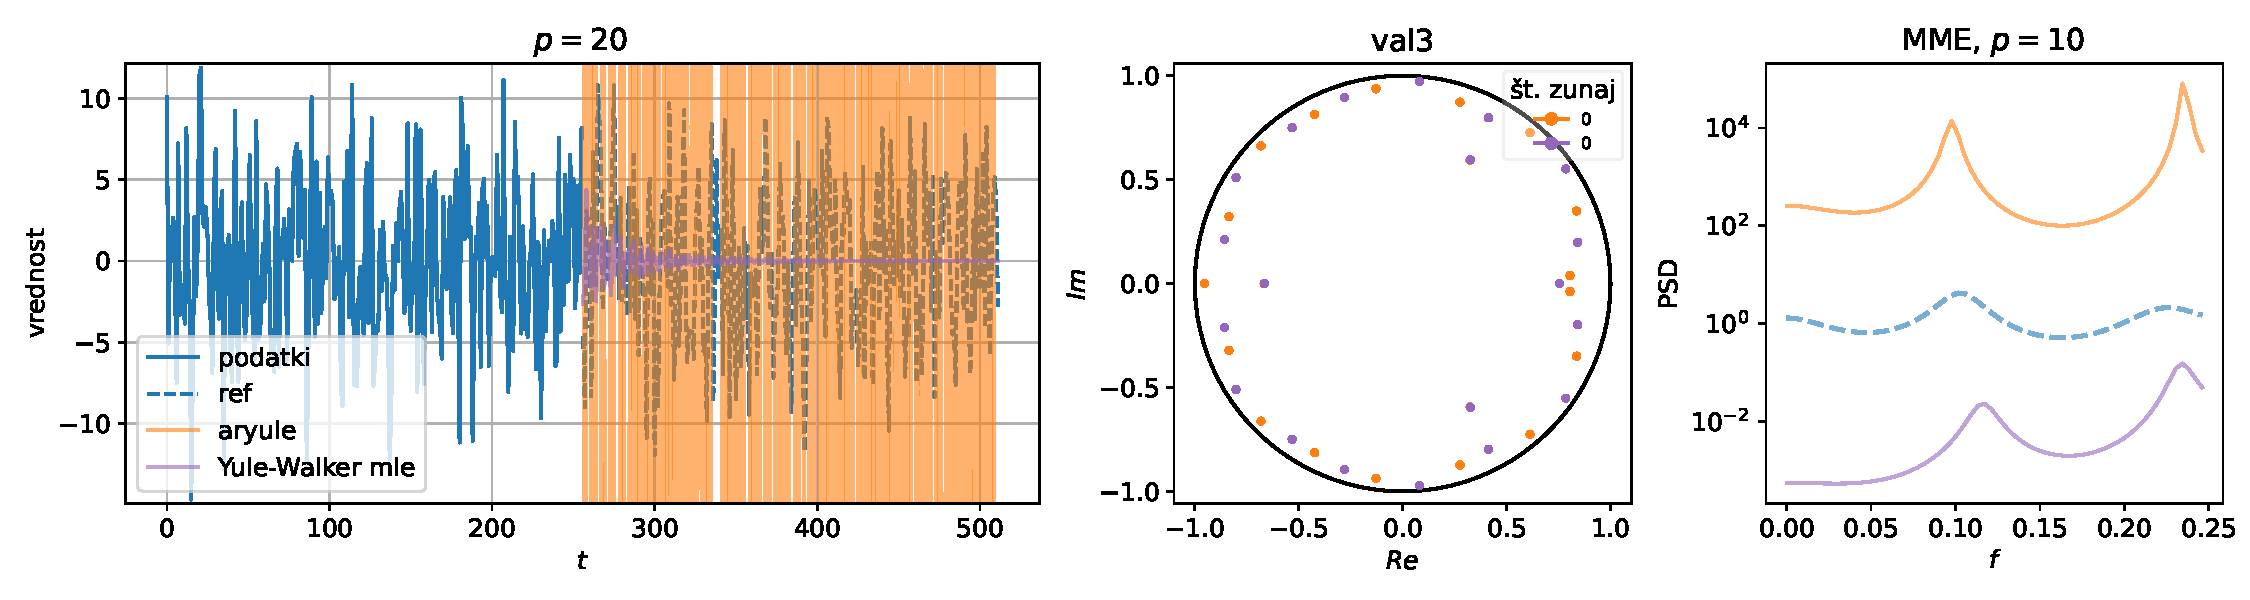
\includegraphics[width=\linewidth]{12.nal_slike/val3_šum4.pdf}
        \caption{}
    \end{subfigure}
    \caption[short]{Napoved zašumjenih podatkov signala val3 z RMS (a) 1, (b) 2 in (c) 4}
\end{figure}

\newpage
\subsection{Dodatek: Temperatura}

Poizkusimo napovedati še en lep vsakdanji primer cikličnega dogajanja: letni in dnevni potek temperature. Poiskal sem po internetu, vendar naš ARSO ne ponuja azhivskih podatko za celotno leto, zato sem na \href{https://www.meteoblue.com/en/weather/archive/export?daterange=2023-01-01%20-%202024-01-01&locations%5B%5D=basel_switzerland_2661604&domain=ERA5T&min=2023-01-01&max=2024-02-15&params%5B%5D=&params%5B%5D=temp2m&params%5B%5D=&params%5B%5D=&params%5B%5D=&params%5B%5D=&params%5B%5D=&params%5B%5D=&params%5B%5D=&utc_offset=%2B00%3A00&timeResolution=hourly&temperatureunit=CELSIUS&velocityunit=KILOMETER_PER_HOUR&energyunit=watts&lengthunit=metric&degree_day_type=10%3B30&gddBase=10&gddLimit=30}{spletni strani} našel (zastonj) podatke o temperaturi, vzorčeni vsako uro za celotno leto v Baslu v Švici. Ker za nek dan v decembru ni bilo podatkov, sem moral luknjo interpolirati. Na PSD spektru letnih temperatur lahko opazimo vrhov, ki ustrezajo značilnim časovnim periodam.

\begin{figure}[ht]
    \begin{subfigure}{0.49\textwidth}
        \centering
        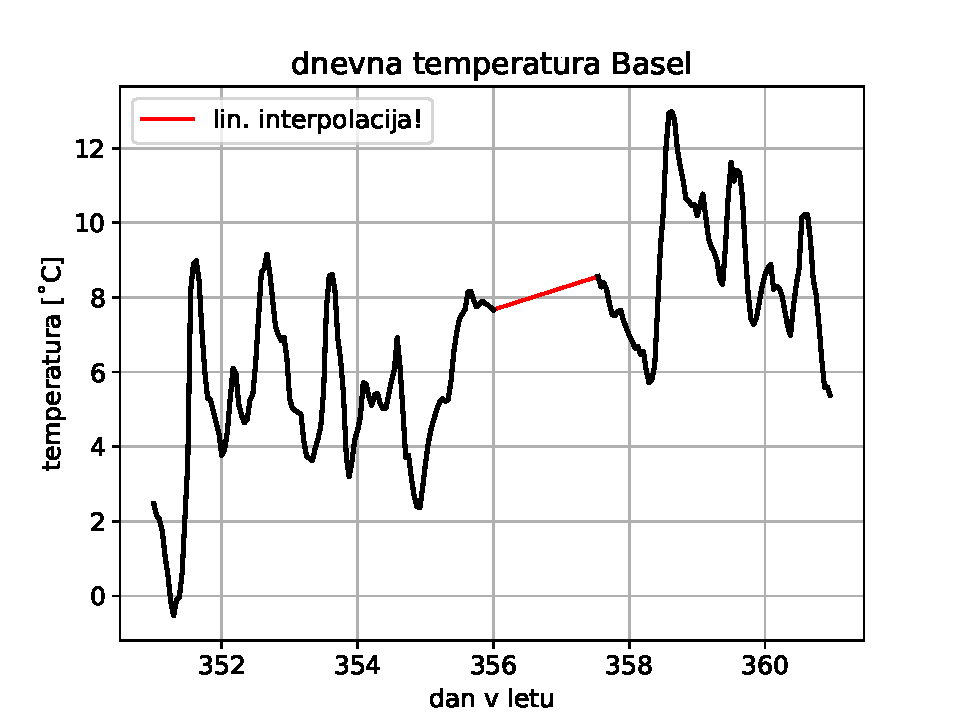
\includegraphics[width=\linewidth]{12.nal_slike/12.1/dnevna_temp.pdf}
        \caption{}
    \end{subfigure}
    \begin{subfigure}{0.49\textwidth}
        \centering
        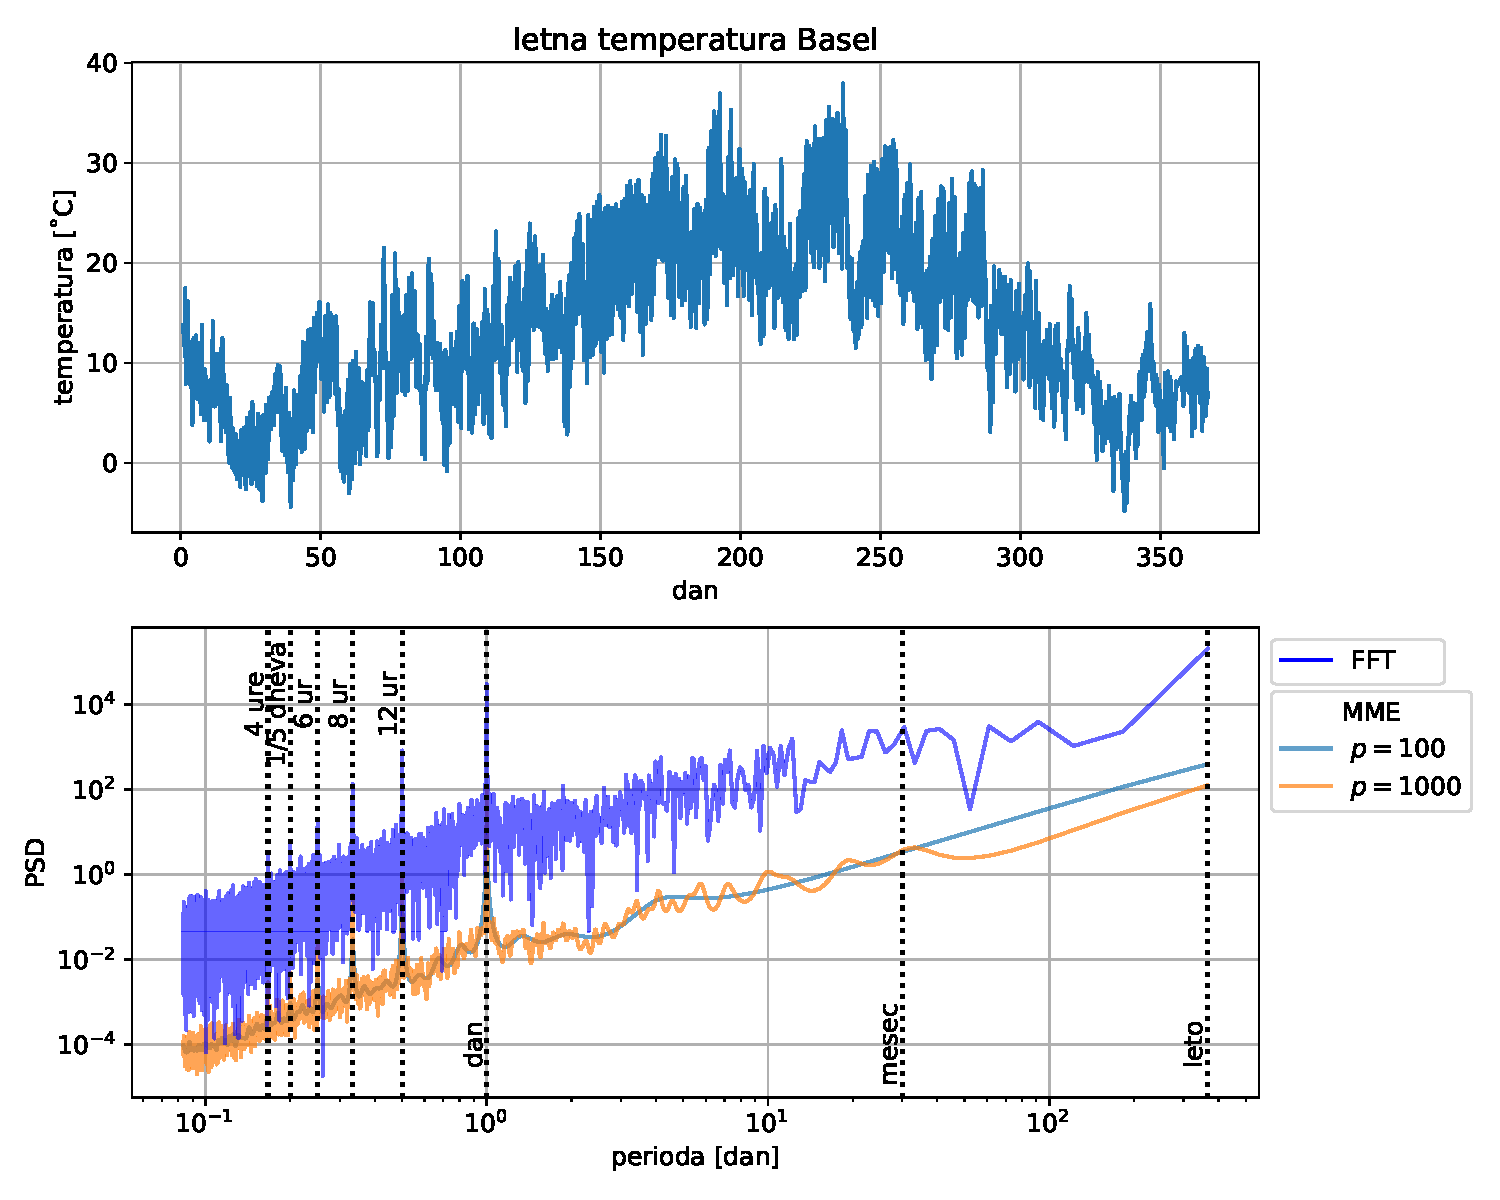
\includegraphics[width=\linewidth]{12.nal_slike/12.1/letna_temp_PSD.pdf}
        \caption{}
    \end{subfigure}
    \caption[short]{Potek (a) dnevnih in (b) letnih temperatur v Baslu, Švica ter PSD}
\end{figure}

Poskusil sem napovedati temperaturo na nekaj prihodnjih dni, vendar ne ravno uspešno. Dnevno periodo sicer zadanemo, vendar se zatakne pri amplitudi nihanja in tedenskem trendu nihanja temperature. Večanje reda je sicer nekoliko bolj uspešno. 6 in 8 urne periodike na tem intervalu niso zaznavne.

\begin{figure}[ht]
    \centering
    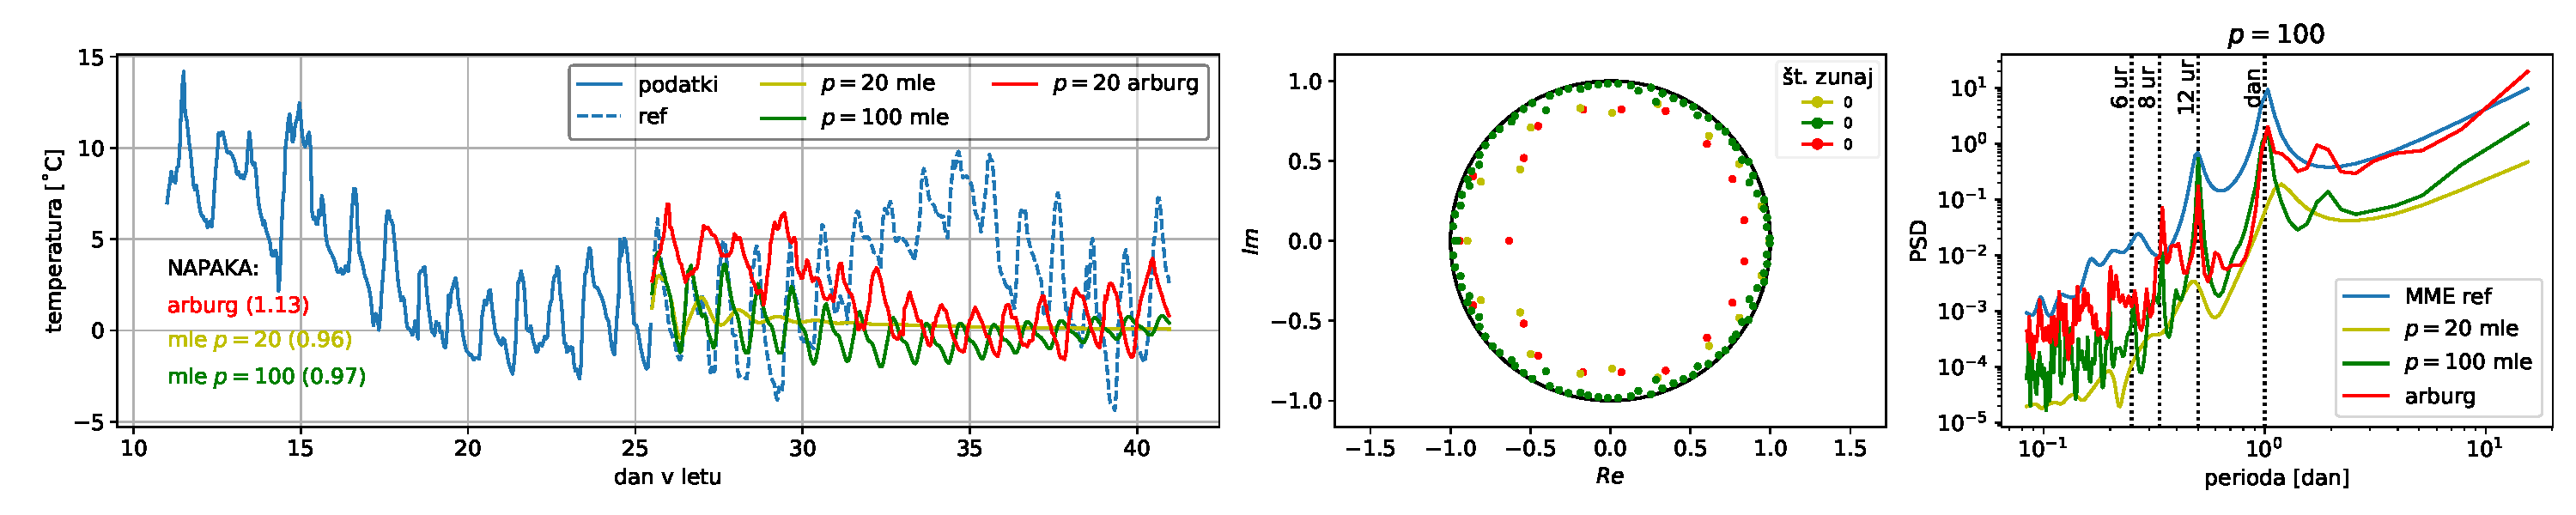
\includegraphics[width=\linewidth]{12.nal_slike/temp_dnevna_napoved.pdf}
    \caption{Napoved dnevne temperature v Baslu}
\end{figure}